\chapter{Background}

\section{Neutron Transport}

Neutron transport is the study of the motion and interactions of neutrons in matter. Neutrons interact with the nuclei of matter and can be absorbed or scattered, depending on the properties of the matter. Neutrons can also leak through a boundary, having passed through matter without being absorbed. Absorption of a neutron leads to one less neutron in the system. The scattering of a neutron does not remove the neutron from the system but rather changes its energy and direction. If a neutron causes fission, it is lost. However, the fission of nuclei lead to the production of neutrons in the system. This accounting of the number of neutrons present in a system at a specific time leads to the fundamental equation of neutron transport, the linear Boltzmann transport equation:
\begin{multline}
	\bigg [ \frac{1}{v(E)} \frac{\partial}{\partial t} + \hat{\Omega} \cdot \nabla + \sigma(\vec{r},E) \bigg ] \psi(\vec{r},\hat{\Omega},E,t) \\ = \int_{0}^{\infty} \diff E' \, \int_{4\pi} \diff \hat{\Omega} \, \sigma_{s}(\vec{r},E'\rightarrow E,\hat{\Omega}' \cdot \hat{\Omega}) \psi(\vec{r},\hat{\Omega}',E',t) \\ + \int_{0}^{\infty} \diff E' \, \nu(E') \chi(E'\rightarrow E) \sigma_{f}(\vec{r},E') \int_{4\pi} \diff \hat{\Omega}' \, \psi(\vec{r},\hat{\Omega}',E',t), 
	\label{eq:NeutronTransport}
\end{multline}
where the quantities are located at position $\vec{r}$, traveling in direction $\hat{\Omega}$, and at energy $E$, and $\sigma$, $\sigma_{s}$, $\sigma_{f}$, and $v$ are the total, scattering, fission macroscopic cross sections, and neutron velocity, respectively. $\chi(E'\rightarrow E)$ is the fission spectrum and specifies the energy distribution of neutrons born from fission and $\nu(E)$ is the average number of neutrons emitted in fission when the neutron causing fission has energy $E$. The angular flux, denoted by $\psi(\vec{r},\hat{\Omega},E,t)$, gives the number of neutrons per unit length squared per steradian per energy per unit time and is the unknown distribution we are looking to solve for. The streaming term of Eq.~\ref{eq:NeutronTransport} can be rewritten using the angle space shown in Figure~\ref{fig:angle_space}. If the direction vector $\hat{\Omega}$ is given by
\begin{equation}
	\hat{\Omega} = \mu \hat{x} + \eta \hat{y} + \xi \hat{z},
\end{equation}
where $\hat{x}, \hat{y},$ and $\hat{z}$ are unit vectors, then it follows that the streaming term is given by
\begin{equation}
	 \hat{\Omega} \cdot \nabla \psi(\vec{r},\hat{\Omega},E,t) = \mu \frac{\partial \psi}{\partial x} + \eta \frac{\partial \psi}{\partial y} + \xi \frac{\partial \psi}{\partial z}.
\end{equation}
The linear Boltzmann transport equation is used in solving many problems in nuclear engineering \cite{duderstadt_nuclear_1976}. We refer to the linear Boltzmann transport equation as the neutron transport equation for the rest of this dissertation. The neutron transport equation is an integro-differential equation for the neutron angular flux and is a function of seven independent variables: three spatial variables, two direction variables, energy, and time.

\begin{figure}
	\centering
	\tdplotsetmaincoords{60}{110}
	
	\pgfmathsetmacro{\rvec}{1.8}
	\pgfmathsetmacro{\thetavec}{40}
	\pgfmathsetmacro{\phivec}{50}
	
	\begin{tikzpicture}[scale=5,tdplot_main_coords]
	
	\coordinate (O) at (0,0,0);
	
	\draw[thick,->] (0,0,0) -- (1,0,0) node[anchor=north east]{$x$};
	\draw[thick,->] (0,0,0) -- (0,1,0) node[anchor=north west]{$y$};
	\draw[thick,->] (0,0,0) -- (0,0,1) node[anchor=south]{$z$};
	
	\tdplotsetcoord{P}{\rvec}{\thetavec}{\phivec}
	\tdplotsetcoord{Q}{1.93}{\thetavec}{\phivec}
	\draw[-stealth,color=black, very thick] (O) -- (P);
	\draw[dashed, color=black, very thick] (O) -- (Pxy);
	\draw[dashed, color=black, very thick] (P) -- (Pxy);
	
	\draw[dashed, color=black, very thick] (0.743717,0,0) -- (Pxy);
	\draw[dashed, color=black, very thick] (0,0.886327,0) -- (Pxy);
	
	\tdplotdrawarc{(O)}{0.3}{0}{\phivec}{anchor=north}{$\cos^{-1}(\mu)$}
	
	\tdplotdrawarc{(O)}{0.4}{50}{90}{anchor=north}{}
	
	\tdplotsetthetaplanecoords{\phivec}\tdplotdrawarc[tdplot_rotated_coords]{(0,0,0)}{0.5}{0}%
		{\thetavec}{anchor=south}{}
	
	\tdplotsetrotatedcoords{\phivec}{\thetavec}{0}
	\tdplotsetrotatedcoordsorigin{(P)}
	
	\draw node at (0,0.2,0.6) {$\cos^{-1}(\xi)$};
	\draw node at (0,0.4,0.1) {$\cos^{-1}(\eta)$};
	
	\draw node at (Q) {$\hat{\Omega}$};
	
	\end{tikzpicture}
	\caption{Neutron Direction Angle Space}
	\label{fig:angle_space} 
\end{figure}

%\begin{figure}
%	\centering
%\tdplotsetmaincoords{60}{120} 
%\begin{tikzpicture} [scale=3, tdplot_main_coords, axis/.style={->,black,thick}, 
%vector/.style={-stealth,black,very thick}, 
%vector guide/.style={dashed,black,thick}]
%
%%standard tikz coordinate definition using x, y, z coords
%\coordinate (O) at (0,0,0);
%
%%tikz-3dplot coordinate definition using x, y, z coords
%
%\pgfmathsetmacro{\ax}{0.8}
%\pgfmathsetmacro{\ay}{0.8}
%\pgfmathsetmacro{\az}{1.2}
%
%\coordinate (P) at (\ax,\ay,\az);
%
%%draw axes
%\draw[axis] (0,0,0) -- (1.5,0,0) node[anchor=north east]{$x$};
%\draw[axis] (0,0,0) -- (0,1.5,0) node[anchor=north west]{$y$};
%\draw[axis] (0,0,0) -- (0,0,1.5) node[anchor=south]{$z$};
%
%%draw a vector from O to P
%\draw[vector] (O) -- (P);
%
%%draw guide lines to components
%\draw[vector guide]         (O) -- (\ax,\ay,0);
%\draw[vector guide] (\ax,\ay,0) -- (P);
%\draw[vector guide]         (P) -- (0,0,\az);
%\draw[vector guide] (\ax,\ay,0) -- (0,\ay,0);
%\draw[vector guide] (\ax,\ay,0) -- (0,\ay,0);
%\draw[vector guide] (\ax,\ay,0) -- (\ax,0,0);
%
%\end{tikzpicture}
%\caption{Neutron Direction Angle Space}
%\label{fig:angle_space} 
%\end{figure}

Solving the neutron transport equation with appropriate initial conditions and boundary conditions yields the expected number of neutrons within a geometry as a function of space, direction, energy, and time. However, the neutron transport equation for neutrons is an integro-differential equation and in general, few analytic solutions exist \cite{lewis_computational_1984}. For this reason, it necessary to use numerical methods to solve practical problems. For neutron transport, there are two classes of computational methods: deterministic and Monte Carlo. In deterministic methods, the position, direction, energy, and time phase space of the transport equation is discretized and a system of equations solved iteratively. Approaches such as the discrete ordinates method where the neutron transport equation is solved along ordinates and quadrature is used to approximate integrals in angle and diamond differencing in space are used to approximate derivative and integral quantities. This discretization process introduces truncation errors and the discretization of irregular geometries can be problematic. In addition, deterministic methods require appropriately homogenized in space and energy nuclear cross sections for system materials which introduces another source of error due to the averaging process. Monte Carlo methods treat the phase space as continuous, allowing for the detailed modeling of geometry and use of continuous cross section data. The Monte Carlo method does not solve the transport equation directly, instead it stochastically simulates the transport of a finite number of neutrons through the problem geometry \cite{lux_monte_1991}. After obtaining a large number of particle interaction histories, averages of particle interactions are extracted, giving the number of neutrons in some part of the phase space, the number of reactions occuring, and other important physical values, within some uncertainty. Monte Carlo methods introduce stochastic uncertainty and can require large number of particle simulations to achieve acceptable uncertainties on calculated parameters.

\section{The Criticality Problem of Neutron Transport}

The ability to fission certain nuclei with neutrons to produce additional neutrons leads to the criticality problem. Given a system with a certain material composition and geometry, is it possible to have a self-sustaining chain reaction? If a system is capable of a self-sustaining chain reaction, we call this system critical, where the loss and production of neutrons are perfectly in balance, allowing the neutron population to be constant in time. If the system is unable to sustain a chain reaction, the system to said to be subcritical. If the neutron population in the system grows without bound, the system is said to be supercritical \cite{bell_nuclear_1970}. It is rare to immediately find a system geometry or material composition that is critical. Instead, some parameter is introducted into the transport equation that forces the system to be critical. Given the sign or magnitude of this parameter, we can judge how far a system is from critical and whether or not the system is subcritical or supercritical. This parameter is the eigenvalue for which we solve numerically. There is no unique way to form an eigenvalue problem \cite{ronen_comparison_1976}, and depending on the application, one eigenvalue formulation may be more useful than others \cite{cacuci_eigenvalue-dependent_1982}. In this dissertation we focus on the $\alpha$- and $k$-eigenvalue problems due to their widespread use in nuclear engineering applications.

\subsection{The Alpha-Eigenvalue Problem}
If we are interested in the time asymptotic behavior of neutron flux in a system, the alpha-eigenvalue problem gives the exponential time-dependent flux behavior and criticality eigenpair of the system \cite{bell_nuclear_1970}. The time asymptotic behavior of the neutron flux is given by the sign of the eigenvalue, which determines whether or not the neutron flux decays to zero, remains constant in time, or grows without bound. We derive the alpha-eigenvalue problem by attempting to solve Eq.~\ref{eq:NeutronTransport} for some initial condition $\psi_{0}(\vec{r},E,\hat{\Omega},t=0)$ and vacuum boundary conditions \cite{lewis_computational_1984}. Defining the operator $A$ as
\begin{multline}
A \equiv v(E) \bigg [ \frac{\chi(E)}{4\pi} \int_{4\pi} \diff \hat{\Omega}' \, \int_{0}^{\infty} \diff E' \, \nu(E) \sigma_{f}(\vec{r},E',t) \\ +\int_{4\pi} \diff \hat{\Omega}' \, \int_{0}^{\infty} \diff E' \sigma_{s}(\vec{r},E'\rightarrow E, \hat{\Omega}' \rightarrow \hat{\Omega},t) - \hat{\Omega} \cdot \nabla - \sigma(\vec{r},E,t) \bigg ],
\end{multline}
we can write the initial value problem as 
\begin{equation}
\frac{\partial \psi}{\partial t} = A \psi.
\label{eq:ivp}
\end{equation}
We expect the previous equation to have solutions in the form of
\begin{equation}
		\psi = \psi_{0} e^{\alpha t},
\end{equation}
where we obtain the eigenvalues $\alpha$ from the equation
\begin{equation}
\alpha \psi = A \psi.
\label{eq:ivp_A}
	\end{equation}
Obtaining the solution of the time-dependent neutron transport equation becomes a matter of determining the eigenvalues (spectrum) of $A$ \cite{bell_nuclear_1970}. Taking the Laplace transform of Eq.~\ref{eq:ivp}, we define
\begin{equation}
	\psi_{\alpha} \equiv \int_{0}^{\infty} \diff t \, e^{\alpha t} \psi(\vec{r},E,\hat{\Omega},t), 
\end{equation}
and obtain
\begin{equation}
	\alpha \psi_{\alpha} - \psi_{0} = A \psi_{\alpha} \rightarrow (\alpha - A) \psi_{\alpha} = \psi_{0}.	\end{equation}
To solve this equation we invert the left-hand side of the previous equation (resolvent operator) and obtain
\begin{equation}
	\psi_{\alpha} = (\alpha - A)^{-1}\psi_{0}.
\end{equation}
Applying the inverse Laplace transform, we obtain the solution to the initial value problem
\begin{equation}
	\psi = \frac{1}{2\pi i} \int_{b - i\infty}^{b + i\infty} \diff \alpha \, (\alpha - A)^{-1}\psi_{0} e^{\alpha t}.
	\label{eq:IVPSoln}
\end{equation}
Equation \ref{eq:IVPSoln} is the formal solution of Eq.~\ref{eq:ivp}. However, this solution still requires that we perform a complex contour integral. To integrate the solution, we must know where the singularities of the integrand operator are located. Assume the operator has a discrete number of poles, then the integral can be performed by extending and closing the contour path to pick up all residue contributions as can be seen in Figure~\ref{fig:Contour}.

\begin{figure}
\centering
\resizebox{0.5\textwidth}{!}{
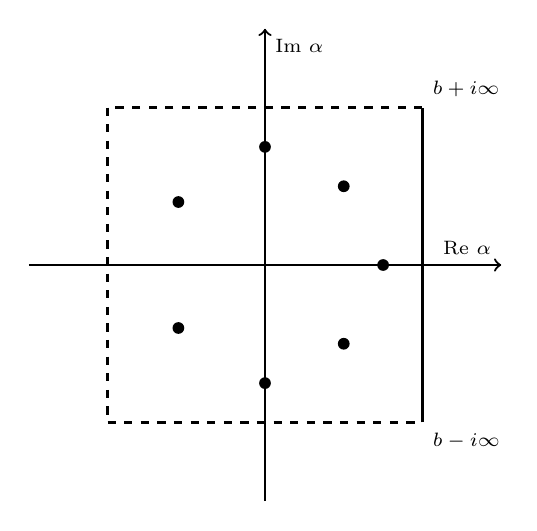
\begin{tikzpicture}
    \begin{scope}[thick,font=\scriptsize]
    % Axes:
    % Are simply drawn using line with the `->` option to make them arrows:
    % The main labels of the axes can be places using `node`s:
    \draw [->] (-3,0) -- (3,0) node [above left]  {Re $\alpha$};
    \draw [->] (0,-3) -- (0,3) node [below right] {Im $\alpha$};

    \draw [-] (2,-2) -- (2,2) node [above right] {$b + i \infty$};
    \draw [dashed] (2,2) -- (-2,2);
    \draw [dashed] (-2,2) -- (-2,-2);
    \draw [dashed] (-2,-2) -- (2,-2) node [below right] {$b - i\infty$};

    %\draw (1,0) node[cross, rotate=45] {};
    \draw (1,1) node[circle, fill, inner sep = 1.5pt] {};
    \draw (1,-1) node[circle, fill, inner sep = 1.5pt] {};
    \draw (-1.1,0.8) node[circle, fill, inner sep = 1.5pt] {};
    \draw (-1.1,-0.8) node[circle, fill, inner sep = 1.5pt] {};
    \draw (1.5,0) node[circle, fill, inner sep = 1.5pt] {};
    \draw (0,1.5) node[circle, fill, inner sep = 1.5pt] {};
    \draw (0,-1.5) node[circle, fill, inner sep = 1.5pt] {};

    \end{scope}
\end{tikzpicture}}
\caption{Contour Integration in Complex Plane of the Operator $A$}
\label{fig:Contour}
\end{figure}

Defining
\begin{equation}
f(\alpha) = (\alpha - A)^{-1}\psi_{0} e^{\alpha t},
\end{equation}
the solution to the initial value problem can be expressed as
\begin{equation}
	\psi = \frac{1}{2\pi i} \int_{b - i\infty}^{b + i\infty} \diff \alpha \, f(\alpha) = \oint_{C} \diff \alpha \, f(\alpha) = 2 \pi i \sum_{k=1}^{n} \text{Res}(f(\alpha),\alpha_{k}).
	\label{eq:IVPsol}
\end{equation}
where $\alpha_{k}$ are the eigenvalues from Eqn.~\ref{eq:ivp_A}. While Eq.~\ref{eq:IVPsol} is the general solution for the initial value problem, usually we are only interested in the asymptotic time solution since at long times it is expected that only the dominant eigenvalue and fundamental mode will remain. Rather than taking the Laplace Transform of Eq.~\ref{eq:ivp}, the $\alpha$-eigenvalue problem is formed by assuming the angular flux solution is separable in time, giving the asymptotic solution
\begin{equation}
	\psi(\vec{r},\hat{\Omega},E,t) = \psi(\vec{r},\hat{\Omega},E) \exp(\alpha t).
\end{equation}
Substituting the asymptotic solution into the neutron transport equation (Equation \ref{eq:NeutronTransport}) yields the $\alpha$-eigenvalue neutron transport equation:
\begin{multline}
	\bigg [ \frac{\alpha}{v(E)} + \hat{\Omega} \cdot \nabla + \sigma(\vec{r},E) \bigg ] \psi(\vec{r},\hat{\Omega},E) \\ = \int \diff E' \, \int \diff \hat{\Omega}' \, \sigma_{s}(\vec{r},E'\rightarrow E,\hat{\Omega}' \cdot \hat{\Omega}) \psi(\vec{r},\hat{\Omega}',E') \\ + \int \diff E' \, \nu(E') \chi(E'\rightarrow E) \sigma_{f}(\vec{r},E') \int \diff \hat{\Omega}' \, \psi(\vec{r},\hat{\Omega}',E').
	\label{eq:AlphaEigEqn}
\end{multline}
We define the operator form of Eq.~\ref{eq:AlphaEigEqn} as
\begin{equation}
(\mathcal{H} + \alpha \mathcal{V}^{-1}) \psi = ( \mathcal{S} + \mathcal{F} ) \psi,
\label{eq:OpFormAlpha}
\end{equation}
where the operators are continuous and given by
\begin{equation}
	\begin{split}
		& \mathcal{H} = \hat{\Omega} \cdot \nabla + \sigma(\vec{r},E), \\
		& \mathcal{V}^{-1} = \frac{1}{v(E)}, \\
		& \mathcal{S} = \int \diff E' \, \int \diff \hat{\Omega} \, \sigma_{s}(\vec{r},E'\rightarrow E,\hat{\Omega}' \cdot \hat{\Omega}) \psi(\vec{r},\hat{\Omega}',E'), \\
		& \mathcal{F} = \int \diff E' \, \nu(E') \chi(E'\rightarrow E) \sigma_{f}(\vec{r},E') \int \diff \hat{\Omega}' \, \psi(\vec{r},\hat{\Omega}',E').
	\end{split}
\end{equation}

In general, there will be a spectrum of eigenvalues for which there are solutions to Equation \ref{eq:AlphaEigEqn} but at long times, only a unique, positive eigenvector, $\psi_{0}$,  corresponding to the algebraically largest eigenvalue, $\alpha_{0}$, remains. The asymptotic solution can be written as \cite{nelkin_asymptotic_1963}
\begin{equation}
	\psi_{\text{asym}}(\vec{r},\hat{\Omega},E,t) \propto \psi_{0}(\vec{r},\hat{\Omega},E) \exp(\alpha_{0} t).
\end{equation}
The criticality of the system can be defined by the sign of $\alpha_{0}$

	$$ \alpha_{0} \begin{cases}						  			  			 > 0, \quad \text{supercritical,} \\			 			 			 = 0, \quad \text{critical,} \\
					 < 0, \quad \text{subcritical.} 					                       \end{cases} $$
The fundamental eigenvalue and eigenvector are real ($\alpha_{0} \in \mathbb{R}, \psi_{0} \in \mathbb{R}^{N}$) but any of the higher eigenvalues and eigenvectors may be negative and complex. 
The $\alpha$-eigenvalues are ordered by their real part
\begin{equation}
	\alpha_{0} > Re(\alpha_{1}) \geq Re(\alpha_{2}) \geq \dots \geq Re(\alpha_{n}).
\end{equation}
Let $\mathcal{T}$ be the transport operator defined as
\begin{equation}
	\mathcal{T} = \mathcal{V}(\mathcal{S}+\mathcal{F} - \mathcal{H}),
\end{equation}
then it follows that the eigenvalue problem can be written as
\begin{equation}
	\alpha \psi = \mathcal{T} \psi.
\end{equation}
Since complex eigenvalues are possible in the spectrum for the real transport operator $\mathcal{T}$, it follows that the complex conjugate of these eigenvalues are also in the spectrum. We prove this as follows:
\begin{theorem}
If there exists a complex eigenvalue in the spectrum, then its complex conjugate is also in the spectrum.
\end{theorem}
\begin{proof}
	Consider the linear transport operator $\mathcal{T} \in \mathbb{R}$. If $\lambda \in \mathbb{C}$ is a complex eigenvalue of $\mathcal{T}$ and $v \in \mathbb{C}^{n}$ is a non-zero eigenfunction of $\mathcal{T}$, then by definition
	\begin{equation}
		\mathcal{T} v = \lambda v.
		\label{eq:ComConj}
	\end{equation}
Taking the complex conjugate of Equation \ref{eq:ComConj} yields
\begin{equation}
	\overline{\mathcal{T}}\overline{v} = \mathcal{T} \overline{v} = \overline{\lambda}\overline{v},
	\end{equation}
since $\mathcal{T}$ is real and linear.
\end{proof}
In addition, given the entire set of eigenvalue and eigenvectors for this eigenvalue problem, any initial condition angular flux can be expressed as a combination of the eigenvectors and eigenvalues. These eigenvalues $\alpha$ exist for systems without fissile material and have units of inverse time as they give a characteristic time of the slowest neutron to leak or be absorbed in the system. In the literature, these eigenvalues are also know as natural, time \cite{hill_efficient_1983}, or $\lambda$ \cite{duderstadt_nuclear_1976} eigenvalues. For simple problems such as one-speed slabs and multigroup-in-energy slab and spherical problems, various features of the $\alpha$-eigenvalue spectrum have been identified. We discuss these results in Section~\ref{sec:AlphaSpec}. It must be noted that the existence of a fundamental eigenvalue is not guaranteed for all problems. In particular, optically thin slabs have been shown to have no fundamental eigenvalue \cite{kornreich_timeeigenvalue_2005}. In contrast to incredibly subcritical problems, for incredibly supercritical systems, two real, positive eigenvalues have been observed \cite{kornreich_timeeigenvalue_2005}. In general, the existence of a sole dominant eigenvalue has also yet to be proven for all cases of interest.

\subsubsection{The Alpha-Eigenvalue Spectrum}
\label{sec:AlphaSpec}

In this section we examine previous work on the $\alpha$-eigenvalue spectrum. Initial examination of the spectrum by Lehner and Wing \cite{lehner_spectrum_1955} for the linear transport operator $\mathcal{T}$ assumed the one-speed, slab geometry form
\begin{equation}
	\mathcal{T}(x,\mu) = -\mu \frac{\partial}{\partial x} + \frac{c}{2} \int_{-1}^{1} \diff \mu'.
\end{equation}
where
\begin{equation}
	c = \frac{\bar{\nu} \sigma_{f} + \sigma_{s}}{\sigma}.
\end{equation}
%It was found that for this particular case, the spectrum only consists of a few discrete eigenvalues. 
Additional studies by J{\"o}rgens extended the spectral analysis to multi-energy media \cite{jorgens_asymptotic_1958}. Larsen extended the spectral analysis to more general geometries \cite{larsen_spectrum_1974} and the multigroup neutron transport operator for bounded spatial domains \cite{larsen_spectrum_1979}. Larsen found that the spectrum of $\mathcal{T}$ for more general problems consists of points, line, and in some cases, a continuum of eigenvalues. An example of the spectrum of $\mathcal{T}$ can be seen in Figure \ref{fig:AlphaEigSpectrum}. The spectrum of $\mathcal{T}$ includes more scalars than just the $\alpha$-eigenvalues. The $\alpha$-eigenvalues are the point and line spectrum of $\mathcal{T}$ \cite{duderstadt_transport_1979}. The point spectrum is finite, all-real set lying in the positive half-plane $\lambda > -\lambda^{*}$, where $\lambda^{*}$ is the minimum value of $v\sigma(v)$. The features of the spectrum of $\mathcal{T}$ are highly dependent on the type of problem being examined. For example, for slab geometry problems, the continuum of eigenvalue occurs due to the possibility a neutron can travel parallel to one of the faces indefinitely before scattering or leaving the slab \cite{wing_transport_1962}. The continuous spectrum is contained in the negative half-plane Re $\lambda \le -\lambda^{*}$. The dividing limit, $-\lambda^{*}$, called the Corngold limit, marks the minimum physically-possible $\alpha$-eigenvalue.

\begin{theorem}
	The Corngold limit, $-\lambda^{*} = -v\sigma(v)$, is the minimum physically possible $\alpha$-eigenvalue.
\end{theorem}

\begin{proof}
	We use the facts that the $\alpha$- and $k$-eigenvalue problems are equal for an exactly critical system and the eigenfunctions corresponding to these eigenvalues are equal \cite{velarde_analysis_1978}. Consider the infinite-medium, one energy group eigenvalue problems:
	\begin{equation}
		\sigma \phi = \sigma_{s} \phi + \frac{\bar{\nu}\sigma_{f}}{k_{\infty}} \phi,
	\end{equation}
	\begin{equation}
		\frac{\alpha_{\infty}}{v}\phi = \sigma_{s} \phi + \bar{\nu}\sigma_{f}\phi - \sigma \phi,
	\end{equation}
where $\bar{\nu}$ is the average number of neutrons emitted in fission and $k_{\infty}$ and $\alpha_{\infty}$ are the infinite-medium $k$-effective and alpha-eigenvalues, respectively. Dividing out the fluxes and combining the two equations yields a relationship for the two eigenvalues for the infinite-medium, one-group problem \cite{kornreich_timeeigenvalue_2005}
\begin{equation}
	\frac{\alpha_{\infty}}{v\sigma} = (k_{\infty}-1) \bigg ( 1 - \frac{\sigma_{s}}{\sigma} \bigg ).
\label{eq:kinfalpha}
\end{equation}
The minimum possible $\alpha$-eigenvalue occurs when there is no fissile material ($k_{\infty} = 0$) or scattering ($\sigma_{s} = 0$) present. Substitution of these values into Equation \ref{eq:kinfalpha} yields
\begin{equation}
	\alpha_{\infty} = - v \sigma = -\lambda^{*},
\end{equation}
which is the Corngold limit.
\end{proof}

The minimum velocity, $v_{\text{min}}$, has interesting impacts on the spectrum of the operator $\mathcal{T}$. Studies on finite media problems where the mimimum velocity is greater than zero ($v_{\text{min}} > 0$) show that the continuous part of the spectrum disappears \cite{jorgens_asymptotic_1958}. Instead of a continuous spectrum, point and line spectra fill the half-space. If the minimum neutron velocity is allowed to approach small speeds, $v_{\text{min}} = 0$, the continuous part of the spectrum reappears. The presence of line spectra results from considering the continuous dependence of the $\alpha$-eigenvalues on neutron velocity. As the velocity varies from some $v$ to $v_{\text{min}}$, some eigenvalues trace out curves in the complex plane or remain stationary \cite{larsen_spectrum_1974}.

Studies suggest that the case where the minimum neutron velocity is bounded away from zero is the more physically valid representation. As the neutron velocity minimum is allowed to go to zero, the neutron wavelength is comparable to the mean free path, thus rendering the neutron transport equation invalid \cite{duderstadt_nuclear_1976}. In this disseration, the neutron transport equation is discretized and energy-dependent cross sections are bounded away from zero. $\alpha$-eigenvalue spectra will then contain only point spectra.

\begin{figure}
	\centering
	\resizebox{0.5\textwidth}{!}{
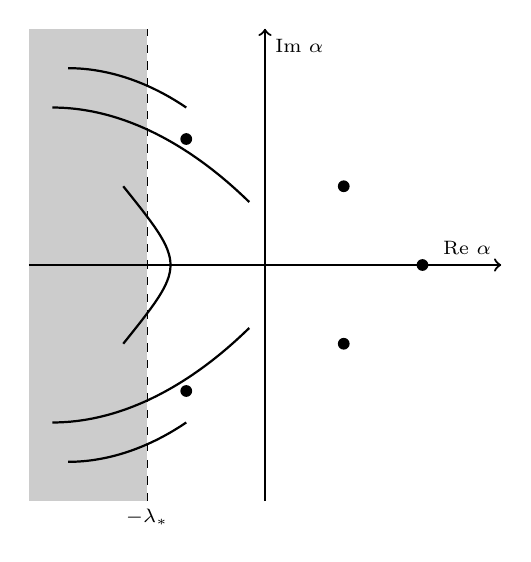
\begin{tikzpicture}
    \begin{scope}[thick,font=\scriptsize]
    % Axes:
    % Are simply drawn using line with the `->` option to make them arrows:
    % The main labels of the axes can be places using `node`s:

    \draw [dashed] (-1.5,-3) -- (-1.5,3) {};

    \draw node at (-1.5,-3.2) {$-\lambda_{*}$};

    \fill[fill=black!20] (-3,-3) rectangle (-1.5,3);
    \draw [->] (-3,0) -- (3,0) node [above left]  {Re $\alpha$};
    \draw [->] (0,-3) -- (0,3) node [below right] {Im $\alpha$};

    \draw (-2.5,2.5) parabola (-1.0,2.0);
    \draw (-2.5,-2.5) parabola (-1.0,-2.0);
    \draw (-2.7,2) parabola (-0.2,0.8);
    \draw (-2.7,-2) parabola (-0.2,-0.8);

    \draw (-1.8,1) .. controls (-1,0) .. (-1.8,-1);

    \draw (1,1) node[circle, fill, inner sep = 1.5pt] {};
    \draw (1,-1) node[circle, fill, inner sep = 1.5pt] {};
    \draw (2,0) node[circle, fill, inner sep = 1.5pt] {};
    \draw (-1,1.6) node[circle, fill, inner sep = 1.5pt] {};
    \draw (-1,-1.6) node[circle, fill, inner sep = 1.5pt] {};

    \end{scope}
\end{tikzpicture}

	}
	\caption{Example Spectrum of the Transport Operator for the One-Speed Slab Geometry Problem}
	\label{fig:AlphaEigSpectrum}
\end{figure}

\subsubsection{Applications of the Alpha-Eigenvalue}

The alpha-eigenvalue and its corresponding eigenvector give the time-dependence of the neutron flux in a nuclear system of interest. For subcritical problems, given some external source, the alpha-eigenvalue measures the length of time necessary for all neutrons to leave the system. One type of system of interest is accelerator-driven subcritical (ADS) systems. ADS systems are subcritical configurations containing multiplying material that are pulsed with a large number of neutrons. These neutrons are generated by an accelerator colliding protons or ions onto a spallation target creating large amounts of neutrons \cite{abderrahim2001myrrha}. ADS systems have received renewed interest because of their ability to address nuclear reactor waste disposal concerns. These systems are able to transmute radioactive isotopes to stable or shorter half-life isotopes by fissioning the radioactive nuclei of concern using high-energy spallation neutrons. The transmutation of long-lived actinides and fission products provide an alternative to geological disposal. Also, the fissioning of nuclei in the system can provide enough power to supply the accelerator, making ADS systems self-sustainable.

The alpha-eigenvalue and eigenvector are necessary to characterize the neutron flux time and spatial variation when the ADS system is in a subcritical state. With the addition of spallation neutrons into the system, the alpha-eigenvalue describes the length of time necessary for the neutron flux to decay. Knowledge of the spatial and time variations in the neutron flux also allows designers to determine the efficient placement of actinides and other fission products in the system for optimal consumption.

%For critical problems, the neutron flux distribution at long times is given by the eigenvector corresponding to the alpha-eigenvalues. 

Another application of the alpha-eigenvalue is for nuclear systems that are supercritical for short periods of time like fast-burst nuclear reactors. Fast-burst reactors generate high-flux neutron pulses that are used in materials radiation testing, electronic hardware hardening testing, and other applications. These supercritical systems return to a subcritical state through some sort of feedback, either geometric or thermal. Since the neutron flux is a time-dependent function, the alpha-eigenvalue gives a measure of the growth rate of the neutron flux. For purely supercritical systems, the neutron flux increases without bound in time and the alpha-eigenvalue measures the $e$-folding time, the time required by the exponentially growing neutron population to increase by a factor of $e$ \cite{duderstadt_nuclear_1976}. To see this, consider Eq.~\ref{eq:kinfalpha}
\begin{equation*}
	\frac{\alpha_{\infty}}{v\sigma} = (k_{\infty}-1) \bigg ( 1 - \frac{\sigma_{s}}{\sigma} \bigg ).
\end{equation*}
Multiplying by $v\sigma$ and using the relation $\sigma_{a} = \sigma - \sigma_{s}$ , we can write
\begin{equation}
	\alpha_{\infty} = v(\nu \sigma_{f} - \sigma_{a}).
\end{equation}
Noting that $k_{\infty} = \bar{\nu} \sigma_{f} / \sigma_{a}$ and the neutron lifetime is given by $\ell = 1/v\sigma_{a}$, we obtain
\begin{equation}
	\alpha_{\infty} = \frac{k_{\infty} - 1}{\ell}.
	\label{eq:alphamax}
\end{equation}
The time rate change of the number of neutrons $N(t)$ in an infinite medium is given by the ordinary differential equation
\begin{equation}
\frac{dN}{dt} = \frac{(k_{\infty} - 1)}{\ell} N(t),
\end{equation}
with solution
\begin{equation}
	N(t) = N_{0} \exp \bigg [ \frac{k_{\infty}-1}{\ell} t \bigg ].
	\label{eq:Nt}
\end{equation}
Comparing the relationship for $\alpha_{\infty}$ and Eq.~\ref{eq:Nt}, we see that we can write
\begin{equation}
	N(t) = N_{0} \exp (\alpha_{\infty} t).
\end{equation}
Relating $\alpha_{\infty}$ to the reactor period $T$ ($e$-folding time), we see that
\begin{equation}
	T = \frac{1}{\alpha_{\infty}}.
\end{equation}
We also note that Eq.~\ref{eq:alphamax} gives the maximum time eigenvalue for a homogeneous system \cite{kornreich_timeeigenvalue_2005}. Higher alpha-eigenvalues are used in reactor kinetics to determine neutron flux responses to reactivity insertions and feedback mechanisms \cite{modak_scheme_2007}. We only focus on the dominant eigenvalue in this dissertation, however, since we are interested in the criticality of nuclear systems.

\subsubsection{Calculating the Alpha-Eigenvalue}
\label{sec:CalcAlpha}

In this section we describe various numerical methods use to determine the alpha-eigenvalue and eigenvector in discrete ordinates neutron transport codes. 
%These methods are used to benchmark the correctness and performance of the Rayleigh Quotient Fixed Point method for alpha-eigenvalue problems. 
Methods other than those described in this section exist and this by no means is a full review of all methods. However, the methods presented here are those used predominantly in neutron transport codes or methods used to determine analytical eigenvalues and eigenvectors for benchmarking.

\textit{The Critical Search Method}: The workhorse method in neutron transport codes for the numerical solution of the the alpha-eigenvalue problem is the critical search method \cite{hill_efficient_1983}. The critical search method is the primary alpha-eigenvalue solver for supercritical problems in codes such as ARDRA \cite{hanebutte_ardra_1999} and PARTISN \cite{alcouffe2005partisn}. For Eq.~\ref{eq:CritSearch}, the critical search performs multiple $k$-effective calculations for various values of $\alpha$:
\begin{multline}
	\bigg [ \frac{\alpha^{\ell}}{v(E)}  + \hat{\Omega} \cdot \nabla + \sigma(\vec{r},E) \bigg ] \psi(\vec{r},\hat{\Omega},E,t) \\ = \int \diff E' \, \int \diff \hat{\Omega}' \, \sigma_{s}(\vec{r},E'\rightarrow E,\hat{\Omega}' \cdot \hat{\Omega}) \psi(\vec{r},\hat{\Omega}',E',t) \\ + \frac{1}{k^{\ell}}\int \diff E' \, \nu(E') \chi(E'\rightarrow E) \sigma_{f}(\vec{r},E') \int \diff \hat{\Omega}' \, \psi(\vec{r},\hat{\Omega}',E',t), 
	\label{eq:CritSearch}
\end{multline}
where $\alpha^{\ell}$ and $k^{\ell}$ are the alpha- and $k$-effective eigenvalues at iteration $\ell$.
The critical search method is described in Algorithm~\ref{algo:critsearch}. Using various guessed values for the alpha-eigenvalue, intermediate $k$-effective eigenvalue calculations are done. The true alpha-eigenvalue is then found by extrapolation using the ($\alpha$, $k$) pairs to find the alpha-eigenvalue such that the system is exactly critical. This extrapolation might require multiple iterations to bracket the eigenvalue. 

In this method, the alpha-eigenvalue introduces artificial absorption into the problem. For sufficiently subcritical systems, negative absorption is possible, potentially causing solution methods to diverge \cite{hill_efficient_1983}. For systems close to critical, many interpolations/extrapolations of alpha-eigenvalue iterates are required and the critical search method might become unacceptably slow. In addition, for systems close to critical, the intermediate $k$-effective calculation convergence might become slow, increasing the cost of the method in the intermediate stage. The question of how converged the $k$-effective eigenvalue calculations must be remains open. Using unconverged $k$-effective eigenvalues in the estimation of the alpha-eigenvalue may slow down or prevent the convergence to the true alpha-eigenvalue. For an eigenvalue that is too tightly converged, iterations are wasted and the method becomes inefficient.

\begin{algorithm}[H]
				\caption{Critical Search Method \cite{hill_efficient_1983}}
				\begin{algorithmic}[1]
					\STATE Make an initial guess for $\alpha^{0}$.
					\STATE Solve Eq. \ref{eq:CritSearch} for $k^{0}$.
					\STATE Obtain a second guess $\alpha^{1}$ by adjusting $\alpha^{0}$ by some eigenvalue modifier value: $\alpha^{1} = \alpha^{0} + \text{EMV}$.
					\STATE Solve Eq.~\ref{eq:CritSearch} for $k^{1}$.
					\WHILE{$\abs{k^{\ell} - 1}/k^{\ell}$ > tolerance}
					\STATE{Using ($\alpha^{\ell}, k^{\ell}$) and ($\alpha^{\ell-1},k^{\ell-1}$), perform a linear extrapolation of $k(\alpha)$ to find $\alpha^{\ell+1}$ such that $k^{\ell+1}(\alpha^{\ell+1}) = 1$.}
					\STATE{Solve Eq. \ref{eq:CritSearch} for $k^{\ell+1}$.}
					\ENDWHILE
					%\STATE Repeat until $k^{\ell+1} = 1$.
				\end{algorithmic}
				\label{algo:critsearch}
\end{algorithm}

\textit{Green's Function Method (GFM)}: Green's Function Method \cite{kornreich_timeeigenvalue_2005} uses Green's functions to model one-speed, multiplying, multi-region slabs and obtain boundary flux values for an eigenvalue search. The one-group neutron transport equation for a homogeneous material with isotropic scattering is
\begin{equation}
	\bigg [ \mu \frac{\partial}{\partial x} + \sigma + \frac{\alpha}{v} \bigg ] \psi(x,\mu) = \frac{\nu \sigma_{f} + \sigma_{s}}{2} \int_{-1}^{-1} \diff \mu' \, \psi(x,\mu').
	\label{eq:GFMNTE}
\end{equation}
Dividing by the total cross section we obtain
\begin{equation}
	\bigg [ \frac{\mu}{\sigma} \frac{\partial}{\partial x} + \alpha' \bigg ] \psi(x,\mu) = \frac{c}{2} \int_{-1}^{1} \diff \mu' \, \psi(x,\mu'),
	%\bigg [ \mu \frac{\partial}{\partial \Delta} + \alpha' \bigg ] \psi(\Delta,\mu) = \frac{c}{2} \int_{-1}^{1} \diff \mu' \, \psi(\Delta,\mu'),
	\label{eq:MFPNTE}
\end{equation}
where
\begin{equation}
	\alpha' = 1 + \frac{\alpha}{v \sigma} \quad \text{and} \quad c = \frac{\nu \sigma_{f} + \sigma_{s}}{\sigma}.
\end{equation}
Eq.~\ref{eq:MFPNTE} is measured in mean free paths. For infinite-medium problems, $\alpha' \geq 0$. This can be seen by allowing $\alpha$ to be the Corngold limit, the smallest possible alpha-eigenvalue, and evaluating for $\alpha'$.

The GFM is useful for multi-region systems because of Placzek's lemma \cite{case1953introduction}. Placzek's lemma states that the angular flux solution in a finite slab can be expressed in terms of a solution in an infinite medium by converting boundary angular flux sources into equivalent volumetric sources. Using the lemma, each slab region can be treated as an infinite homogeneous medium with a specified source based on the angular flux boundary conditions. For an infinite medium, the angular flux can be expressed by the Green's function
\begin{equation}
\psi(x,\mu) = \int_{-\infty}^{\infty} \diff x' \, \int_{-1}^{1} \diff \mu' \, \big [ \mu' \psi(0,\mu') \delta(x') - \mu' \psi(\Delta,\mu') \delta(x'-\Delta,\mu') \big]  G(x-x', \mu | \mu'),
\end{equation}
where the Green's function satisfies the integro-differential equation
\begin{equation}
	\bigg [ \mu \frac{\partial}{\partial x} + \alpha' \bigg ] G(x,\mu \mid \mu') = \frac{c}{2} \int_{-1}^{1} \diff \mu'' \, G(x,\mu'' \mid \mu') + \delta(x) \delta(\mu - \mu'),
	\label{eq:GreenIntegroDiff}
\end{equation}
and $\Delta$ is the width of the finite slab in mean free paths.

The solution, $G(x,\mu \mid \mu')$, to Eq.~\ref{eq:GreenIntegroDiff} is in the form of the solution to the anisotropic plane source emitting particles in direction $\mu'$ for an infinite homogeneous medium problem with scattering parameter $c$. Taking a Fourier transform of Eq.~\ref{eq:GreenIntegroDiff}, integrating over the scattering angle $\mu$, inverting the transform, and using Placzek's lemma to connect individual slab regions through boundary angular fluxes, an integral equation for the angular flux in the multi-region medium is found:
\begin{align}
\begin{split}
	\psi_{i}&(0^{+}, -\mu) + \int_{0}^{1} \diff \mu' \, \mu' \psi_{i}(0^{+}, - \mu') \big [ G_{c}(0^{-}, \mu \mid \mu') \pm G_{c}(-\Delta_{i}, -\mu' \mid \mu') \big ] \\
	&\pm \psi_{i}(\Delta_{i}^{-},\mu) \pm \int_{0}^{1} \diff \mu' \, \mu' \psi_{i}(\Delta_{i}^{-}, \mu') \big [ G_{c}(0^{-}, \mu \mid \mu') \pm G_{c}(-\Delta_{i}, -\mu \mid \mu') \big ] \\
	&\mp \psi_{i-1}(\Delta_{i-1}^{-}, \mu) \exp \bigg ( \frac{-\alpha' \Delta_{i}}{\mu} \bigg ) - \int_{0}^{1} \diff \mu' \, \mu' \psi_{i-1}(\Delta_{i-1}^{-}, \mu') \big [ G_{c}(0^{+}, -\mu \mid \mu') \\
	&\pm G_{c}(\Delta_{i}^{-}, \mu \mid \mu') \big ] - \psi_{i+1}(0^{+}, -\mu) \exp \bigg ( \frac{-\alpha' \Delta_{i}}{\mu} \bigg ) \\
	&\mp \int_{0}^{1} \diff \mu' \, \mu' \psi_{i+1}(0^{+}, -\mu') \big [ G_{c}(0^{+}, -\mu \mid \mu') \pm G_{c}(\Delta_{i}^{-}, \mu \mid \mu') \big ] = 0,
\end{split}
\label{eq:GFMBC}
\end{align}
where
\begin{equation}
	G_{c}(x, \mu \mid \mu') = \frac{c}{2\alpha'} \frac{1}{\mu' - \mu} \big [ h(x,\mu') - h(x,\mu) \big ],
\end{equation}
\begin{equation}
	h(x,\mu) = \frac{\mu}{2\pi} \int_{-\infty}^{\infty} \diff k \, \frac{e^{ikx}}{\alpha' + i k \mu} \frac{1}{1 - \frac{c}{\alpha'} L \big ( \frac{k}{\alpha'} \big ) },
\end{equation}
and
\begin{equation}
	L(z) = \frac{1}{2} \int_{-1}^{1} \diff \mu \, \frac{1}{1 + i z \mu} = \frac{\tan^{-1} z}{z}.
\end{equation}

The eigenvalue problem is formulated by construction of a matrix of the interactions of slab boundary angular fluxes for each region as given by Eq.~\ref{eq:GFMBC}. The matrix consists of submatrices for each region where the integrals are approximated using numerical quadrature. Eigenvalues are then determined using a brute force search routine where all possible values for the eigenvalue within some search space are tested until a value is found such that the real and imaginary parts of the matrix determinant are zero. This value is then the eigenvalue of the system. GFM allows for the calculation of higher eigenvalues and eigenmodes. GFM provides benchmark-quality calculations for the alpha-eigenvalues in heterogeneous media slab problems.

The increase of computational difficulty increases with the number of regions present in the system. In addition, the search space might become large, especially if there is no estimate of the eigenvalue. The numerical quadrature of the integrals also present another cost, as improper integrals must be approximated in each region of the problem to some tolerance. Determination of the matrix determinant requires a complex LU decomposition routine. Further, the scope of GFM is limited to slab geometry, though by using the slab-spherical equivalence \cite{case1953introduction} the eigenvalues of one-dimensional spherical systems can be determined by solving an equivalent slab geometry problem when certain conditions are met.

\textit{Direct Evaluation}: Another numerical method capable of obtaining the alpha-eigen\-value and higher eigenvalues involves forming the matrix problem from the discretized form of the one-speed, one-dimensional transport equation \cite{modak_simple_2003} using discrete ordinates in angle and diamond differencing in space. Using a process similar to the one described in Chapter~\ref{Discrete} with $M$ directions in angle and $N$ cells in space yields a generalized eigenvalue problem of the form
\begin{equation}
\mathbf{A} \psi = \alpha \mathbf{B} \psi.
\label{eq:geneig}
\end{equation}
Using standard eigenvalue solvers, the method gives $NM$ eigenpairs. Given the discretization of the problem, the method gives far more eigenvalues than expected from theory as the discretization process introduces additional eigenvalues that are artifacts from the discretization process. The spectrum is composed of the real eigenvalue spectrum and additional eigenvalues which are a product of the discretization of the problem. An example spectrum can be seen in Figure~\ref{fig:NMSpec}. If only the dominant eigenvalue and vector are required, the formation of the matrices and the eigenvalue solver could be too costly. Direct evaluation works well for homogeneous and multi-region slabs with isotropic scattering. However, the method quickly becomes complicated and expensive for problems involving complex geometries, anisotropic scattering, and multiple energy groups.

\begin{figure}
\centering
\resizebox{0.5\textwidth}{!}{
	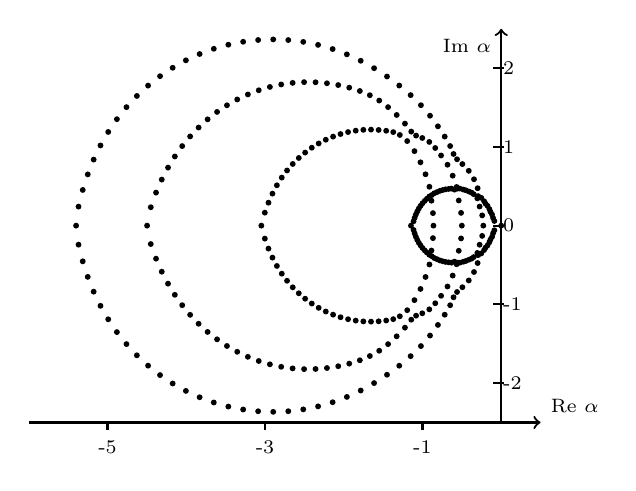
\begin{tikzpicture}
    \begin{scope}[thick,font=\scriptsize]
    % Axes:
    % Are simply drawn using line with the `->` option to make them arrows:
    % The main labels of the axes can be places using `node`s:
    \draw [->] (-6,-2.5) -- (0.5,-2.5) node [above right]  {Re $\alpha$};
    \draw [->] (0,-2.5) -- (0,2.5) node [below left] {Im $\alpha$};

\draw (-5.398972, 0.000000) node [circle, fill, inner sep = 0.75pt] {}; 
\draw (-5.368051, 0.241653) node [circle, fill, inner sep = 0.75pt] {}; 
\draw (-5.368051, -0.241653) node [circle, fill, inner sep = 0.75pt] {}; 
\draw (-5.314660, 0.453320) node [circle, fill, inner sep = 0.75pt] {}; 
\draw (-5.314660, -0.453320) node [circle, fill, inner sep = 0.75pt] {}; 
\draw (-5.250899, 0.650726) node [circle, fill, inner sep = 0.75pt] {}; 
\draw (-5.250899, -0.650726) node [circle, fill, inner sep = 0.75pt] {}; 
\draw (-5.176049, 0.838730) node [circle, fill, inner sep = 0.75pt] {}; 
\draw (-5.176049, -0.838730) node [circle, fill, inner sep = 0.75pt] {}; 
\draw (-5.089480, 1.018392) node [circle, fill, inner sep = 0.75pt] {}; 
\draw (-5.089480, -1.018392) node [circle, fill, inner sep = 0.75pt] {}; 
\draw (-4.991031, 1.189624) node [circle, fill, inner sep = 0.75pt] {}; 
\draw (-4.991031, -1.189624) node [circle, fill, inner sep = 0.75pt] {}; 
\draw (-4.880867, 1.351921) node [circle, fill, inner sep = 0.75pt] {}; 
\draw (-4.880867, -1.351921) node [circle, fill, inner sep = 0.75pt] {}; 
\draw (-4.759369, 1.504612) node [circle, fill, inner sep = 0.75pt] {}; 
\draw (-4.759369, -1.504612) node [circle, fill, inner sep = 0.75pt] {}; 
\draw (-4.627079, 1.646972) node [circle, fill, inner sep = 0.75pt] {}; 
\draw (-4.627079, -1.646972) node [circle, fill, inner sep = 0.75pt] {}; 
\draw (-4.484664, 1.778266) node [circle, fill, inner sep = 0.75pt] {}; 
\draw (-4.484664, -1.778266) node [circle, fill, inner sep = 0.75pt] {}; 
\draw (-4.332887, 1.897790) node [circle, fill, inner sep = 0.75pt] {}; 
\draw (-4.332887, -1.897790) node [circle, fill, inner sep = 0.75pt] {}; 
\draw (-4.172599, 2.004881) node [circle, fill, inner sep = 0.75pt] {}; 
\draw (-4.172599, -2.004881) node [circle, fill, inner sep = 0.75pt] {}; 
\draw (-4.004716, 2.098935) node [circle, fill, inner sep = 0.75pt] {}; 
\draw (-4.004716, -2.098935) node [circle, fill, inner sep = 0.75pt] {}; 
\draw (-3.830219, 2.179414) node [circle, fill, inner sep = 0.75pt] {}; 
\draw (-3.830219, -2.179414) node [circle, fill, inner sep = 0.75pt] {}; 
\draw (-3.650135, 2.245850) node [circle, fill, inner sep = 0.75pt] {}; 
\draw (-3.650135, -2.245850) node [circle, fill, inner sep = 0.75pt] {}; 
\draw (-3.465534, 2.297857) node [circle, fill, inner sep = 0.75pt] {}; 
\draw (-3.465534, -2.297857) node [circle, fill, inner sep = 0.75pt] {}; 
\draw (-4.497469, 0.000000) node [circle, fill, inner sep = 0.75pt] {}; 
\draw (-3.277516, 2.335126) node [circle, fill, inner sep = 0.75pt] {}; 
\draw (-3.277516, -2.335126) node [circle, fill, inner sep = 0.75pt] {}; 
\draw (-3.087206, 2.357434) node [circle, fill, inner sep = 0.75pt] {}; 
\draw (-3.087206, -2.357434) node [circle, fill, inner sep = 0.75pt] {}; 
\draw (-4.450482, 0.233771) node [circle, fill, inner sep = 0.75pt] {}; 
\draw (-4.450482, -0.233771) node [circle, fill, inner sep = 0.75pt] {}; 
\draw (-4.383755, 0.419347) node [circle, fill, inner sep = 0.75pt] {}; 
\draw (-4.383755, -0.419347) node [circle, fill, inner sep = 0.75pt] {}; 
\draw (-4.310987, 0.584750) node [circle, fill, inner sep = 0.75pt] {}; 
\draw (-4.310987, -0.584750) node [circle, fill, inner sep = 0.75pt] {}; 
\draw (-4.231560, 0.736986) node [circle, fill, inner sep = 0.75pt] {}; 
\draw (-4.231560, -0.736986) node [circle, fill, inner sep = 0.75pt] {}; 
\draw (-2.895744, 2.364643) node [circle, fill, inner sep = 0.75pt] {}; 
\draw (-2.895744, -2.364643) node [circle, fill, inner sep = 0.75pt] {}; 
\draw (-2.704272, 2.356699) node [circle, fill, inner sep = 0.75pt] {}; 
\draw (-2.704272, -2.356699) node [circle, fill, inner sep = 0.75pt] {}; 
\draw (-4.145062, 0.878531) node [circle, fill, inner sep = 0.75pt] {}; 
\draw (-4.145062, -0.878531) node [circle, fill, inner sep = 0.75pt] {}; 
\draw (-4.051379, 1.010384) node [circle, fill, inner sep = 0.75pt] {}; 
\draw (-4.051379, -1.010384) node [circle, fill, inner sep = 0.75pt] {}; 
\draw (-3.950604, 1.132900) node [circle, fill, inner sep = 0.75pt] {}; 
\draw (-3.950604, -1.132900) node [circle, fill, inner sep = 0.75pt] {}; 
\draw (-3.842981, 1.246116) node [circle, fill, inner sep = 0.75pt] {}; 
\draw (-3.842981, -1.246116) node [circle, fill, inner sep = 0.75pt] {}; 
\draw (-3.728873, 1.349901) node [circle, fill, inner sep = 0.75pt] {}; 
\draw (-3.728873, -1.349901) node [circle, fill, inner sep = 0.75pt] {}; 
\draw (-2.513925, 2.333632) node [circle, fill, inner sep = 0.75pt] {}; 
\draw (-2.513925, -2.333632) node [circle, fill, inner sep = 0.75pt] {}; 
\draw (-3.608732, 1.444041) node [circle, fill, inner sep = 0.75pt] {}; 
\draw (-3.608732, -1.444041) node [circle, fill, inner sep = 0.75pt] {}; 
\draw (-3.483081, 1.528287) node [circle, fill, inner sep = 0.75pt] {}; 
\draw (-3.483081, -1.528287) node [circle, fill, inner sep = 0.75pt] {}; 
\draw (-3.352507, 1.602380) node [circle, fill, inner sep = 0.75pt] {}; 
\draw (-3.352507, -1.602380) node [circle, fill, inner sep = 0.75pt] {}; 
\draw (-2.325810, 2.295553) node [circle, fill, inner sep = 0.75pt] {}; 
\draw (-2.325810, -2.295553) node [circle, fill, inner sep = 0.75pt] {}; 
\draw (-3.217643, 1.666076) node [circle, fill, inner sep = 0.75pt] {}; 
\draw (-3.217643, -1.666076) node [circle, fill, inner sep = 0.75pt] {}; 
\draw (-2.140976, 2.242657) node [circle, fill, inner sep = 0.75pt] {}; 
\draw (-2.140976, -2.242657) node [circle, fill, inner sep = 0.75pt] {}; 
\draw (-3.079162, 1.719153) node [circle, fill, inner sep = 0.75pt] {}; 
\draw (-3.079162, -1.719153) node [circle, fill, inner sep = 0.75pt] {}; 
\draw (-2.937769, 1.761430) node [circle, fill, inner sep = 0.75pt] {}; 
\draw (-2.937769, -1.761430) node [circle, fill, inner sep = 0.75pt] {}; 
\draw (-1.960361, 2.175248) node [circle, fill, inner sep = 0.75pt] {}; 
\draw (-1.960361, -2.175248) node [circle, fill, inner sep = 0.75pt] {}; 
\draw (-2.794191, 1.792764) node [circle, fill, inner sep = 0.75pt] {}; 
\draw (-2.794191, -1.792764) node [circle, fill, inner sep = 0.75pt] {}; 
\draw (-2.649172, 1.813070) node [circle, fill, inner sep = 0.75pt] {}; 
\draw (-2.649172, -1.813070) node [circle, fill, inner sep = 0.75pt] {}; 
\draw (-1.784717, 2.093828) node [circle, fill, inner sep = 0.75pt] {}; 
\draw (-1.784717, -2.093828) node [circle, fill, inner sep = 0.75pt] {}; 
\draw (-2.503465, 1.822328) node [circle, fill, inner sep = 0.75pt] {}; 
\draw (-2.503465, -1.822328) node [circle, fill, inner sep = 0.75pt] {}; 
\draw (-1.614594, 1.999356) node [circle, fill, inner sep = 0.75pt] {}; 
\draw (-1.614594, -1.999356) node [circle, fill, inner sep = 0.75pt] {}; 
\draw (-2.357833, 1.820610) node [circle, fill, inner sep = 0.75pt] {}; 
\draw (-2.357833, -1.820610) node [circle, fill, inner sep = 0.75pt] {}; 
\draw (-2.213083, 1.808118) node [circle, fill, inner sep = 0.75pt] {}; 
\draw (-2.213083, -1.808118) node [circle, fill, inner sep = 0.75pt] {}; 
\draw (-1.450721, 1.893643) node [circle, fill, inner sep = 0.75pt] {}; 
\draw (-1.450721, -1.893643) node [circle, fill, inner sep = 0.75pt] {}; 
\draw (-2.070158, 1.785217) node [circle, fill, inner sep = 0.75pt] {}; 
\draw (-2.070158, -1.785217) node [circle, fill, inner sep = 0.75pt] {}; 
\draw (-1.294957, 1.779129) node [circle, fill, inner sep = 0.75pt] {}; 
\draw (-1.294957, -1.779129) node [circle, fill, inner sep = 0.75pt] {}; 
\draw (-1.930370, 1.752379) node [circle, fill, inner sep = 0.75pt] {}; 
\draw (-1.930370, -1.752379) node [circle, fill, inner sep = 0.75pt] {}; 
\draw (-1.795683, 1.709747) node [circle, fill, inner sep = 0.75pt] {}; 
\draw (-1.795683, -1.709747) node [circle, fill, inner sep = 0.75pt] {}; 
\draw (-3.046314, 0.000000) node [circle, fill, inner sep = 0.75pt] {}; 
\draw (-3.002116, 0.164835) node [circle, fill, inner sep = 0.75pt] {}; 
\draw (-3.002116, -0.164835) node [circle, fill, inner sep = 0.75pt] {}; 
\draw (-2.955943, 0.291515) node [circle, fill, inner sep = 0.75pt] {}; 
\draw (-2.955943, -0.291515) node [circle, fill, inner sep = 0.75pt] {}; 
\draw (-2.905347, 0.406320) node [circle, fill, inner sep = 0.75pt] {}; 
\draw (-2.905347, -0.406320) node [circle, fill, inner sep = 0.75pt] {}; 
\draw (-2.849030, 0.512173) node [circle, fill, inner sep = 0.75pt] {}; 
\draw (-2.849030, -0.512173) node [circle, fill, inner sep = 0.75pt] {}; 
\draw (-1.150385, 1.657504) node [circle, fill, inner sep = 0.75pt] {}; 
\draw (-1.150385, -1.657504) node [circle, fill, inner sep = 0.75pt] {}; 
\draw (-1.668409, 1.656142) node [circle, fill, inner sep = 0.75pt] {}; 
\draw (-1.668409, -1.656142) node [circle, fill, inner sep = 0.75pt] {}; 
\draw (-1.549437, 1.588679) node [circle, fill, inner sep = 0.75pt] {}; 
\draw (-1.549437, -1.588679) node [circle, fill, inner sep = 0.75pt] {}; 
\draw (-2.787051, 0.610032) node [circle, fill, inner sep = 0.75pt] {}; 
\draw (-2.787051, -0.610032) node [circle, fill, inner sep = 0.75pt] {}; 
\draw (-2.719757, 0.700354) node [circle, fill, inner sep = 0.75pt] {}; 
\draw (-2.719757, -0.700354) node [circle, fill, inner sep = 0.75pt] {}; 
\draw (-2.647560, 0.783376) node [circle, fill, inner sep = 0.75pt] {}; 
\draw (-2.647560, -0.783376) node [circle, fill, inner sep = 0.75pt] {}; 
\draw (-2.570879, 0.859210) node [circle, fill, inner sep = 0.75pt] {}; 
\draw (-2.570879, -0.859210) node [circle, fill, inner sep = 0.75pt] {}; 
\draw (-2.490135, 0.927895) node [circle, fill, inner sep = 0.75pt] {}; 
\draw (-2.490135, -0.927895) node [circle, fill, inner sep = 0.75pt] {}; 
\draw (-1.019702, 1.529438) node [circle, fill, inner sep = 0.75pt] {}; 
\draw (-1.019702, -1.529438) node [circle, fill, inner sep = 0.75pt] {}; 
\draw (-1.436793, 1.504923) node [circle, fill, inner sep = 0.75pt] {}; 
\draw (-1.436793, -1.504923) node [circle, fill, inner sep = 0.75pt] {}; 
\draw (-2.405756, 0.989420) node [circle, fill, inner sep = 0.75pt] {}; 
\draw (-2.405756, -0.989420) node [circle, fill, inner sep = 0.75pt] {}; 
\draw (-2.318173, 1.043750) node [circle, fill, inner sep = 0.75pt] {}; 
\draw (-2.318173, -1.043750) node [circle, fill, inner sep = 0.75pt] {}; 
\draw (-2.227829, 1.090838) node [circle, fill, inner sep = 0.75pt] {}; 
\draw (-2.227829, -1.090838) node [circle, fill, inner sep = 0.75pt] {}; 
\draw (-0.000436, 0.000000) node [circle, fill, inner sep = 0.75pt] {}; 
\draw (-0.904289, 1.396147) node [circle, fill, inner sep = 0.75pt] {}; 
\draw (-0.904289, -1.396147) node [circle, fill, inner sep = 0.75pt] {}; 
\draw (-2.135174, 1.130635) node [circle, fill, inner sep = 0.75pt] {}; 
\draw (-2.135174, -1.130635) node [circle, fill, inner sep = 0.75pt] {}; 
\draw (-1.327589, 1.405567) node [circle, fill, inner sep = 0.75pt] {}; 
\draw (-1.327589, -1.405567) node [circle, fill, inner sep = 0.75pt] {}; 
\draw (-2.040669, 1.163101) node [circle, fill, inner sep = 0.75pt] {}; 
\draw (-2.040669, -1.163101) node [circle, fill, inner sep = 0.75pt] {}; 
\draw (-1.944782, 1.188208) node [circle, fill, inner sep = 0.75pt] {}; 
\draw (-1.944782, -1.188208) node [circle, fill, inner sep = 0.75pt] {}; 
\draw (-1.847984, 1.205947) node [circle, fill, inner sep = 0.75pt] {}; 
\draw (-1.847984, -1.205947) node [circle, fill, inner sep = 0.75pt] {}; 
\draw (-1.750762, 1.216335) node [circle, fill, inner sep = 0.75pt] {}; 
\draw (-1.750762, -1.216335) node [circle, fill, inner sep = 0.75pt] {}; 
\draw (-1.653593, 1.219370) node [circle, fill, inner sep = 0.75pt] {}; 
\draw (-1.653593, -1.219370) node [circle, fill, inner sep = 0.75pt] {}; 
\draw (-1.222656, 1.295667) node [circle, fill, inner sep = 0.75pt] {}; 
\draw (-1.222656, -1.295667) node [circle, fill, inner sep = 0.75pt] {}; 
\draw (-1.556737, 1.215160) node [circle, fill, inner sep = 0.75pt] {}; 
\draw (-1.556737, -1.215160) node [circle, fill, inner sep = 0.75pt] {}; 
\draw (-0.803922, 1.261088) node [circle, fill, inner sep = 0.75pt] {}; 
\draw (-0.803922, -1.261088) node [circle, fill, inner sep = 0.75pt] {}; 
\draw (-1.460927, 1.204936) node [circle, fill, inner sep = 0.75pt] {}; 
\draw (-1.460927, -1.204936) node [circle, fill, inner sep = 0.75pt] {}; 
\draw (-1.371071, 1.187849) node [circle, fill, inner sep = 0.75pt] {}; 
\draw (-1.371071, -1.187849) node [circle, fill, inner sep = 0.75pt] {}; 
\draw (-0.717539, 1.131005) node [circle, fill, inner sep = 0.75pt] {}; 
\draw (-0.717539, -1.131005) node [circle, fill, inner sep = 0.75pt] {}; 
\draw (-1.142532, 1.194528) node [circle, fill, inner sep = 0.75pt] {}; 
\draw (-1.142532, -1.194528) node [circle, fill, inner sep = 0.75pt] {}; 
\draw (-1.287783, 1.151467) node [circle, fill, inner sep = 0.75pt] {}; 
\draw (-1.287783, -1.151467) node [circle, fill, inner sep = 0.75pt] {}; 
\draw (-1.081099, 1.143454) node [circle, fill, inner sep = 0.75pt] {}; 
\draw (-1.081099, -1.143454) node [circle, fill, inner sep = 0.75pt] {}; 
\draw (-1.002352, 1.113238) node [circle, fill, inner sep = 0.75pt] {}; 
\draw (-1.002352, -1.113238) node [circle, fill, inner sep = 0.75pt] {}; 
\draw (-1.193864, 1.073825) node [circle, fill, inner sep = 0.75pt] {}; 
\draw (-1.193864, -1.073825) node [circle, fill, inner sep = 0.75pt] {}; 
\draw (-0.648434, 1.010891) node [circle, fill, inner sep = 0.75pt] {}; 
\draw (-0.648434, -1.010891) node [circle, fill, inner sep = 0.75pt] {}; 
\draw (-0.913382, 1.063160) node [circle, fill, inner sep = 0.75pt] {}; 
\draw (-0.913382, -1.063160) node [circle, fill, inner sep = 0.75pt] {}; 
\draw (-0.605405, 0.909813) node [circle, fill, inner sep = 0.75pt] {}; 
\draw (-0.605405, -0.909813) node [circle, fill, inner sep = 0.75pt] {}; 
\draw (-0.837849, 0.985808) node [circle, fill, inner sep = 0.75pt] {}; 
\draw (-0.837849, -0.985808) node [circle, fill, inner sep = 0.75pt] {}; 
\draw (-0.561131, 0.842652) node [circle, fill, inner sep = 0.75pt] {}; 
\draw (-0.561131, -0.842652) node [circle, fill, inner sep = 0.75pt] {}; 
\draw (-0.493057, 0.781756) node [circle, fill, inner sep = 0.75pt] {}; 
\draw (-0.493057, -0.781756) node [circle, fill, inner sep = 0.75pt] {}; 
\draw (-0.087187, 0.059053) node [circle, fill, inner sep = 0.75pt] {}; 
\draw (-0.087187, -0.059053) node [circle, fill, inner sep = 0.75pt] {}; 
\draw (-0.103489, 0.097354) node [circle, fill, inner sep = 0.75pt] {}; 
\draw (-0.103489, -0.097354) node [circle, fill, inner sep = 0.75pt] {}; 
\draw (-1.101787, 0.946150) node [circle, fill, inner sep = 0.75pt] {}; 
\draw (-1.101787, -0.946150) node [circle, fill, inner sep = 0.75pt] {}; 
\draw (-0.412085, 0.695999) node [circle, fill, inner sep = 0.75pt] {}; 
\draw (-0.412085, -0.695999) node [circle, fill, inner sep = 0.75pt] {}; 
\draw (-0.763637, 0.891223) node [circle, fill, inner sep = 0.75pt] {}; 
\draw (-0.763637, -0.891223) node [circle, fill, inner sep = 0.75pt] {}; 
\draw (-0.345688, 0.588734) node [circle, fill, inner sep = 0.75pt] {}; 
\draw (-0.345688, -0.588734) node [circle, fill, inner sep = 0.75pt] {}; 
\draw (-0.227301, 0.000000) node [circle, fill, inner sep = 0.75pt] {}; 
\draw (-0.116331, 0.141339) node [circle, fill, inner sep = 0.75pt] {}; 
\draw (-0.116331, -0.141339) node [circle, fill, inner sep = 0.75pt] {}; 
\draw (-0.136723, 0.176533) node [circle, fill, inner sep = 0.75pt] {}; 
\draw (-0.136723, -0.176533) node [circle, fill, inner sep = 0.75pt] {}; 
\draw (-0.150844, 0.211221) node [circle, fill, inner sep = 0.75pt] {}; 
\draw (-0.150844, -0.211221) node [circle, fill, inner sep = 0.75pt] {}; 
\draw (-0.299645, 0.475287) node [circle, fill, inner sep = 0.75pt] {}; 
\draw (-0.299645, -0.475287) node [circle, fill, inner sep = 0.75pt] {}; 
\draw (-0.173675, 0.251071) node [circle, fill, inner sep = 0.75pt] {}; 
\draw (-0.173675, -0.251071) node [circle, fill, inner sep = 0.75pt] {}; 
\draw (-0.198679, 0.279005) node [circle, fill, inner sep = 0.75pt] {}; 
\draw (-0.198679, -0.279005) node [circle, fill, inner sep = 0.75pt] {}; 
\draw (-0.217085, 0.309610) node [circle, fill, inner sep = 0.75pt] {}; 
\draw (-0.217085, -0.309610) node [circle, fill, inner sep = 0.75pt] {}; 
\draw (-0.252984, 0.352492) node [circle, fill, inner sep = 0.75pt] {}; 
\draw (-0.252984, -0.352492) node [circle, fill, inner sep = 0.75pt] {}; 
\draw (-0.281534, 0.360728) node [circle, fill, inner sep = 0.75pt] {}; 
\draw (-0.281534, -0.360728) node [circle, fill, inner sep = 0.75pt] {}; 
\draw (-1.025338, 0.803995) node [circle, fill, inner sep = 0.75pt] {}; 
\draw (-1.025338, -0.803995) node [circle, fill, inner sep = 0.75pt] {}; 
\draw (-0.682101, 0.773035) node [circle, fill, inner sep = 0.75pt] {}; 
\draw (-0.682101, -0.773035) node [circle, fill, inner sep = 0.75pt] {}; 
\draw (-0.241795, 0.130273) node [circle, fill, inner sep = 0.75pt] {}; 
\draw (-0.241795, -0.130273) node [circle, fill, inner sep = 0.75pt] {}; 
\draw (-0.294159, 0.374575) node [circle, fill, inner sep = 0.75pt] {}; 
\draw (-0.294159, -0.374575) node [circle, fill, inner sep = 0.75pt] {}; 
\draw (-0.274446, 0.242545) node [circle, fill, inner sep = 0.75pt] {}; 
\draw (-0.274446, -0.242545) node [circle, fill, inner sep = 0.75pt] {}; 
\draw (-0.303300, 0.346285) node [circle, fill, inner sep = 0.75pt] {}; 
\draw (-0.303300, -0.346285) node [circle, fill, inner sep = 0.75pt] {}; 
\draw (-0.349161, 0.399422) node [circle, fill, inner sep = 0.75pt] {}; 
\draw (-0.349161, -0.399422) node [circle, fill, inner sep = 0.75pt] {}; 
\draw (-0.377360, 0.419408) node [circle, fill, inner sep = 0.75pt] {}; 
\draw (-0.377360, -0.419408) node [circle, fill, inner sep = 0.75pt] {}; 
\draw (-0.411367, 0.433901) node [circle, fill, inner sep = 0.75pt] {}; 
\draw (-0.411367, -0.433901) node [circle, fill, inner sep = 0.75pt] {}; 
\draw (-0.616302, 0.634292) node [circle, fill, inner sep = 0.75pt] {}; 
\draw (-0.616302, -0.634292) node [circle, fill, inner sep = 0.75pt] {}; 
\draw (-0.449529, 0.448900) node [circle, fill, inner sep = 0.75pt] {}; 
\draw (-0.449529, -0.448900) node [circle, fill, inner sep = 0.75pt] {}; 
\draw (-0.961205, 0.652050) node [circle, fill, inner sep = 0.75pt] {}; 
\draw (-0.961205, -0.652050) node [circle, fill, inner sep = 0.75pt] {}; 
\draw (-0.482929, 0.459082) node [circle, fill, inner sep = 0.75pt] {}; 
\draw (-0.482929, -0.459082) node [circle, fill, inner sep = 0.75pt] {}; 
\draw (-0.527573, 0.470761) node [circle, fill, inner sep = 0.75pt] {}; 
\draw (-0.527573, -0.470761) node [circle, fill, inner sep = 0.75pt] {}; 
\draw (-0.566865, 0.490865) node [circle, fill, inner sep = 0.75pt] {}; 
\draw (-0.566865, -0.490865) node [circle, fill, inner sep = 0.75pt] {}; 
\draw (-0.557555, 0.470353) node [circle, fill, inner sep = 0.75pt] {}; 
\draw (-0.557555, -0.470353) node [circle, fill, inner sep = 0.75pt] {}; 
\draw (-0.500231, 0.000000) node [circle, fill, inner sep = 0.75pt] {}; 
\draw (-0.509962, 0.162284) node [circle, fill, inner sep = 0.75pt] {}; 
\draw (-0.509962, -0.162284) node [circle, fill, inner sep = 0.75pt] {}; 
\draw (-1.146165, 0.000000) node [circle, fill, inner sep = 0.75pt] {}; 
\draw (-0.539186, 0.319354) node [circle, fill, inner sep = 0.75pt] {}; 
\draw (-0.539186, -0.319354) node [circle, fill, inner sep = 0.75pt] {}; 
\draw (-0.911760, 0.493365) node [circle, fill, inner sep = 0.75pt] {}; 
\draw (-0.911760, -0.493365) node [circle, fill, inner sep = 0.75pt] {}; 
\draw (-0.593540, 0.457538) node [circle, fill, inner sep = 0.75pt] {}; 
\draw (-0.593540, -0.457538) node [circle, fill, inner sep = 0.75pt] {}; 
\draw (-0.632457, 0.470382) node [circle, fill, inner sep = 0.75pt] {}; 
\draw (-0.632457, -0.470382) node [circle, fill, inner sep = 0.75pt] {}; 
\draw (-0.667757, 0.466117) node [circle, fill, inner sep = 0.75pt] {}; 
\draw (-0.667757, -0.466117) node [circle, fill, inner sep = 0.75pt] {}; 
\draw (-0.706665, 0.461145) node [circle, fill, inner sep = 0.75pt] {}; 
\draw (-0.706665, -0.461145) node [circle, fill, inner sep = 0.75pt] {}; 
\draw (-0.779890, 0.441491) node [circle, fill, inner sep = 0.75pt] {}; 
\draw (-0.779890, -0.441491) node [circle, fill, inner sep = 0.75pt] {}; 
\draw (-0.743597, 0.452326) node [circle, fill, inner sep = 0.75pt] {}; 
\draw (-0.743597, -0.452326) node [circle, fill, inner sep = 0.75pt] {}; 
\draw (-0.816207, 0.425754) node [circle, fill, inner sep = 0.75pt] {}; 
\draw (-0.816207, -0.425754) node [circle, fill, inner sep = 0.75pt] {}; 
\draw (-0.849843, 0.411238) node [circle, fill, inner sep = 0.75pt] {}; 
\draw (-0.849843, -0.411238) node [circle, fill, inner sep = 0.75pt] {}; 
\draw (-0.860473, 0.000000) node [circle, fill, inner sep = 0.75pt] {}; 
\draw (-1.113169, 0.055036) node [circle, fill, inner sep = 0.75pt] {}; 
\draw (-1.113169, -0.055036) node [circle, fill, inner sep = 0.75pt] {}; 
\draw (-1.099303, 0.099578) node [circle, fill, inner sep = 0.75pt] {}; 
\draw (-1.099303, -0.099578) node [circle, fill, inner sep = 0.75pt] {}; 
\draw (-0.882587, 0.387840) node [circle, fill, inner sep = 0.75pt] {}; 
\draw (-0.882587, -0.387840) node [circle, fill, inner sep = 0.75pt] {}; 
\draw (-1.083993, 0.140929) node [circle, fill, inner sep = 0.75pt] {}; 
\draw (-1.083993, -0.140929) node [circle, fill, inner sep = 0.75pt] {}; 
\draw (-1.066456, 0.179998) node [circle, fill, inner sep = 0.75pt] {}; 
\draw (-1.066456, -0.179998) node [circle, fill, inner sep = 0.75pt] {}; 
\draw (-0.912602, 0.370305) node [circle, fill, inner sep = 0.75pt] {}; 
\draw (-0.912602, -0.370305) node [circle, fill, inner sep = 0.75pt] {}; 
\draw (-0.971316, 0.314778) node [circle, fill, inner sep = 0.75pt] {}; 
\draw (-0.971316, -0.314778) node [circle, fill, inner sep = 0.75pt] {}; 
\draw (-0.943846, 0.341514) node [circle, fill, inner sep = 0.75pt] {}; 
\draw (-0.943846, -0.341514) node [circle, fill, inner sep = 0.75pt] {}; 
\draw (-0.999334, 0.284387) node [circle, fill, inner sep = 0.75pt] {}; 
\draw (-0.999334, -0.284387) node [circle, fill, inner sep = 0.75pt] {}; 
\draw (-1.046450, 0.217099) node [circle, fill, inner sep = 0.75pt] {}; 
\draw (-1.046450, -0.217099) node [circle, fill, inner sep = 0.75pt] {}; 
\draw (-1.023788, 0.251782) node [circle, fill, inner sep = 0.75pt] {}; 
\draw (-1.023788, -0.251782) node [circle, fill, inner sep = 0.75pt] {}; 
\draw (-0.886138, 0.316296) node [circle, fill, inner sep = 0.75pt] {}; 
\draw (-0.886138, -0.316296) node [circle, fill, inner sep = 0.75pt] {}; 
\draw (-0.866934, 0.158784) node [circle, fill, inner sep = 0.75pt] {}; 
\draw (-0.866934, -0.158784) node [circle, fill, inner sep = 0.75pt] {}; 

\foreach \x in {-5,-3,-1}
     		%\draw (\x,1pt) -- (\x,-3pt)
		\draw (\x,-2.5) -- (\x,-2.6)
			node[anchor=north] {\x};
    	\foreach \y in {-2,...,2}
	\draw (1pt,\y) -- (-3pt,\y) 
     			node[anchor=west] {\y}; 
	%labels      
	%\node[below=0.8cm] at (x axis mid) {MOPS};
	%\node[rotate=90, above=0.8cm] at (y axis mid) {Power [mW]};


     \end{scope}
    \end{tikzpicture}
	}
	\caption{Discretized Alpha-Eigenvalue Spectrum for a Subcritical System}
	\label{fig:NMSpec}
\end{figure}

\subsection{The $k$-Effective Eigenvalue}
\label{subsec:k}

In the $k$-effective eigenvalue problem, the time-dependence of the problem is eliminated and it is assumed there is no external source present \cite{bell_nuclear_1970}. Instead, a time-independent solution is obtained by weighting $\nu$ by a parameter $k$, which expresses the deviation from critical. Substituting $\nu/k$ for $\nu$ yields the k-eigenvalue problem: 
\begin{multline}
	\bigg [ \hat{\Omega} \cdot \nabla + \sigma(\vec{r},E) \bigg ] \psi(\vec{r},\hat{\Omega},E) \\ = \int \diff E' \, \int \diff \hat{\Omega} \, \sigma_{s}(\vec{r},E'\rightarrow E,\hat{\Omega}' \cdot \hat{\Omega}) \psi(\vec{r},\hat{\Omega}',E') \\ + \frac{1}{k} \int \diff E' \, \nu(E') \chi(E'\rightarrow E) \sigma_{f}(\vec{r},E') \int \diff \hat{\Omega}' \, \psi(\vec{r},\hat{\Omega}',E').
	\label{eq:kEigEqn}
\end{multline}
We define the operator form of Eq.~\ref{eq:kEigEqn} as
\begin{equation}
\mathcal{H} \psi = \bigg ( \mathcal{S} + \frac{1}{k}\mathcal{F} \bigg ) \psi.
\label{eq:OpFormk}
\end{equation}
For Eq~\ref{eq:OpFormk}, there are multiple eigenvalues and eigenvectors, but the only positive eigenvector corresponds to the largest real eigenvalue, $k_{0}$. The $k$-effective eigenvalue exists for any system containing fissile material and corresponding to the eigenvalue is a non-negative eigenvector. For a system containing no fissile material, the $k$-effective eigenvalue is undefined. The criticality of a system can be defined by the value of $k$:
	$$ k \begin{cases}						  			  			 > 1, \quad \text{supercritical,} \\			 			 			= 1, \quad \text{critical,} \\
					 < 1, \quad \text{subcritical.} 				       \end{cases} $$

The spectrum of eigenvalues for the $k$-effective eigenvalue problem is real and positive. The spectrum is ordered
\begin{equation}
	k_{0} > k_{1} > k_{2} > \dots k_{N},
\end{equation}
where $k_{0} = k$ is the dominant eigenvalue and $N$ is the total number of eigenvalues. An example of a $k$-effective eigenvalue spectrum can be seen in Figure~\ref{fig:keffspec}. The full set of $k$-eigenvalues and eigenvectors have applications in perturbation theory and provide a measure of numerical convergence for methods like the power method \cite{lewis_computational_1984}. The dominance ratio, the ratio $k_{1}/k_{0}$, provides a measure of convergence for the power method, the standard eigensolver for $k$-effective eigenvalue problem in nuclear engineering applications \cite{lewis_computational_1984}. If a designer is interested in how far a system is from a critical configuration, the $k$-effective eigenvalue is a good measure as it represents the ratio between the fission source and losses due to leakage and absorption. For an exactly critical system, the eigenvector corresponding to $k$ is the flux shape within the reactor. For systems close to critical, the eigenvector is a good approximation of the flux shape. The $k$-effective eigenvalue has another simple physical interpretation: it is the ratio of neutrons in the next generation to those in the current generation \cite{ronen_comparison_1976}.

\begin{figure}
	\centering
	\resizebox{0.5\textwidth}{!}{
	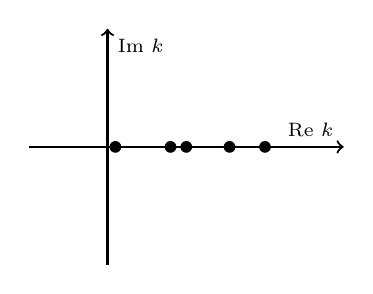
\begin{tikzpicture}
    \begin{scope}[thick,font=\scriptsize]
    % Axes:
    % Are simply drawn using line with the `->` option to make them arrows:
    % The main labels of the axes can be places using `node`s:

    %\draw [dashed] (-1.5,-3) -- (-1.5,3) {};

    %\draw node at (-1.5,-3.2) {$-\lambda_{*}$};

    %\fill[fill=black!20] (-3,-3) rectangle (-1.5,3);
    \draw [->] (-1,0) -- (3,0) node [above left]  {Re $k$};
    \draw [->] (0,-1.5) -- (0,1.5) node [below right] {Im $k$};

    %\draw (-2.5,2.5) parabola (-1.0,2.0);
    %\draw (-2.5,-2.5) parabola (-1.0,-2.0);
    %\draw (-2.7,2) parabola (-0.2,0.8);
    %\draw (-2.7,-2) parabola (-0.2,-0.8);

    %\draw (-1.8,1) .. controls (-1,0) .. (-1.8,-1);

    \draw (1.55,0) node[circle, fill, inner sep = 1.5pt] {};
    \draw (1,0) node[circle, fill, inner sep = 1.5pt] {};
    \draw (2,0) node[circle, fill, inner sep = 1.5pt] {};
    \draw (0.1,0) node[circle, fill, inner sep = 1.5pt] {};
    \draw (0.8,0) node[circle, fill, inner sep = 1.5pt] {};

    \end{scope}
\end{tikzpicture}
	}
	\caption{Example Spectrum for $k$-Effective Eigenvalue}
	\label{fig:keffspec}
\end{figure}

\subsubsection{Iterative Methods for the $k$-Effective Eigenvalue}

In this section we describe two standard iterative methods used to calculate the $k$-effective eigenvalue of a nuclear system, the power method and shifted inverse iteration. As discussed in Section~\ref{subsec:k}, the criticality of the nuclear system is given by the largest real $k$-effective eigenvalue and corresponding to this eigenvalue is the only positive eigenvector. This positive eigenvector is the neutron angular flux of the nuclear system. Discretization of Eq.~\ref{eq:kEigEqn} leads to large sparse linear systems, which makes the use of \textit{direct} eigenvalue solvers (such as the QR method) too expensive or unfeasible. In addition, most transport codes apply the discretized operators of Eq.~\ref{eq:kEigEqn} through matrix-vector multiplication or \textit{transport sweeps}, defined as inversions of the operator $\mathcal{H}$ \cite{willert_comparison_2014}, to invert operators and do not construct the large sparse matrices \cite{lewis_computational_1984}. Given that determining the criticality and fundamental flux mode only requires the dominant eigenvalue, it is instead preferably to use iterative eigenvalue methods.

\textbf{Power Method with Fission Norm Update}: The most basic method for solving for the $k$-effective eigenvalue is the power method \cite{lewis_computational_1984}. To apply the method, we write the $k$-effective criticality problem as the standard eigenvalue problem
\begin{equation}
k \psi = (\mathcal{H} - \mathcal{S})^{-1} \mathcal{F}\psi.
\label{eq:PM}
\end{equation}

The power method, described in Algorithm~\ref{algo:PM}, consists of iteratively applying the operator on the right of Eq.~\ref{eq:PM} to some eigenfunction approximation at iteration $i$, $\psi^{i+1}$. The eigenfunction is then usually normalized by some norm of the angular flux.% such as the total fission rate in the system \cite{warsa_krylov_2004}. 

\begin{algorithm}[H]
				\caption{Power Method \cite{lewis_computational_1984}}
				\begin{algorithmic}[1]
					\STATE{Make initial guess $\psi^{(0)}, k^{(0)}$.}
					\FOR {$i = 0, 1, 2, \cdots,$}
						\STATE{Compute $\psi^{(i+1)} = \frac{1}{k^{(i)}}(\mathcal{H - S})^{-1} \mathcal{F} \psi^{(i)}$}.
						\STATE{Normalize $\psi^{(i+1)}$ by some norm, compute $k^{(i+1)}$.}
						\STATE{Check for convergence: $\abs{k^{(i+1)} - k^{(i)}}/k^{(i+1)}$ < tolerance}
					\ENDFOR
				\end{algorithmic}
				\label{algo:PM}
\end{algorithm}

There are various ways to compute the eigenvalue iterate. One simple estimate of the eigenvalue is given by the expression
\begin{equation}
k^{(i+1)} = k^{(i)} \frac{ \norm{\psi^{(i+1)}}}{\norm{\psi^{(i)}}},
\end{equation}
where $\norm{\psi}$ is some discrete norm taken over the problem domain. However, only a normalization is necessary and a norm is not required. In many implementations the norm takes into account only the isotropic scalar flux component as this is usually the required unknown \cite{warsa2004krylov}. However, there is no mathematical justification for this norm and any consistent norm can be used. Traditionally, in neutron transport codes, the eigenvalue is estimated using the total fission rate in the problem \cite{warsa2004krylov} which is given by 
\begin{equation}
	\norm{\phi} \equiv \norm{\phi}_{F} = \sum_{g=1}^{G} \sum_{s \in \mathcal{D}} \nu \sigma_{f,g,s} \phi_{0,g,s}
\end{equation}
where the summation is over all energy group and over all spatial cells in the problem domain, $\mathcal{D}$. Another possible eigenvalue update is the Rayleigh quotient, where the Rayleigh quotient is defined as
\begin{equation}
	R(M,x) = \frac{x^{T}Mx}{x^{T}x},
\end{equation}
where $M \in \mathbb{R}^{N \times N}$ and $x \in \mathbb{R}^{N \times 1}$ \cite{horn_matrix_2012}. It has been observed that using the Rayleigh quotient can at times improve the efficiency of the power iteration by providing a better estimate of the eigenvalue earlier in the iterative process \cite{warsa2004krylov}.

The power method converges to the eigenvector corresponding to the largest eigenvalue in modulus provided that the eigenvalue is simple and the initial eigenvector guess contains a component in the eigendirection \cite{golub_matrix_2012}. It has been shown that $k$ is the largest eigenvalue in modulus for various types of problems in nuclear engineering \cite{modak_evaluation_1995}. However, it is possible the power iteration will not converge. For instance, for multigroup energy problems, it is not known if the dominant eigenvalue is always real and given an all real initial eigenvector guess, it is possible the method will not converge. In addition, the power method converges with rate equal to the dominance ratio, $k_{1}/k_{0}$, and for problems with dominance ratios close to one, convergence can be unacceptably slow. Problems with dominance ratios close to one include highly scattering nuclear reactor problems such as heavy water reactors and boiling water reactors. Despite these limitations, the simplicity of the power method makes it the default eigenvalue solver method of choice in neutron transport codes \cite{duderstadt_nuclear_1976}.

\textit{The Wielandt Method}: Another method to calculate the $k$-effective eigenvalue is the Wielandt method or Wielandt acceleration (Algorithm~\ref{algo:SII}) \cite{yamamoto_reliable_2004}. The Wielandt method, as it is known in the neutron transport community, is a shifted inverse iteration method \cite{ipsen_computing_1997} applied to the $k$-effective eigenvalue problem. In the shifted inverse iteration method, the power method is applied to the shifted problem of the form
\begin{equation}
(\mathcal{H} - \mathcal{S} - \beta \mathcal{F})\psi = (\lambda - \beta) \mathcal{F} \psi,
\end{equation}
where $\lambda = 1/k$ and the shift $\beta$ is selected such that $0 < \abs{\lambda_{1} - \beta} < \abs{\lambda_{2} - \beta} \leq \abs{\lambda_{j} - \beta}$, $j > 2$. It can be shown that this yields a method with speed of convergence determined by $\abs{\lambda_{1} - \beta}/\abs{\lambda_{2} - \beta}$ \cite{ipsen_computing_1997}. For an appropriately selected shift $\beta$, the method can be faster than the power method. For criticality problems in nuclear engineering, the systems are expected to be close to critical and the shift can be selected to be $\beta = 1$. The power method can be considered a special case of the shifted inverse iteration method with no shift. Despite its improved theoretical convergence rate, the shifted inverse iteration shift requires \textit{a priori} knowledge of the dominant eigenvalue magnitude. Given a poor shift, convergence of the method may be delayed.

\begin{algorithm}[H]
				\caption{Shifted Inverse Iteration \cite{ipsen_computing_1997}}
				\begin{algorithmic}[1]
					\STATE{Make initial guess $\psi^{(0)}$.}
					\FOR{$i = 0, 1, 2, \cdots,$}
						\STATE{Define shift $\beta^{(i)}$}.
						\STATE{Compute $\psi^{(i+1)}$ such that $(\mathcal{H-S} -\beta^{(i)}\mathcal{F}) \psi^{(i+1)}= \mathcal{F}\psi^{(i)}$}.
						\STATE{Normalize $\psi^{(i+1)}$ by some norm.}
						\STATE{Check for Convergence}
					\ENDFOR
				\end{algorithmic}
				\label{algo:SII}
\end{algorithm}


%The alpha- and $k$-eigenvalue problems are equal when the system is critical. The eigenvectors for both problems will be equal and the eigenvalues for an infinite medium, one-group group can be related by Eq.~\ref{eq:kinfalpha} \cite{kornreich_timeeigenvalue_2005}.



%Given a particular application, certain eigenvalue problems can give designers different information. For instance, if a designer seeks the time asymptotic behavior of neutron flux in a system, the $\alpha$-eigenvalue problem gives the exponential time-dependent flux behavior and criticality eigenpair of the system \cite{bell_nuclear_1970}. By assuming that the neutron flux unknown is separable in time, the sign of the eigenvalue determines whether or not the neutron flux decays to zero, remains constant in time, or grows without bound.We discuss the $\alpha$-eigenvalue and $k$-eigenvalue problems in depth in Chapter \ref{ch2}.

\section{Review of Linear Algebra Fundamentals}
\label{sec:LinAlg}

We review and introduce some definitions of linear algebra concepts used in this dissertation. Of particular interest are the concepts of positivity and primitivity, which guide the derivation of the method later in this disseration. Definitions and theorems are from \cite{horn_matrix_2012}, \cite{birkhoff_mathematical_1961}, \cite{varga_matrix_2009}. The theory of Perron-Frobenius for positive, irreducible, and primitive matrices is discussed and its results are used heavily throughout this dissertation.

\subsection{Nonnegativity, Positivity, and the Spectral Radius of a Matrix}

\begin{definition}
A real matrix $\mathbf{A}$ is nonnegative (or positive) if all entries of $\mathbf{A}$ are nonnegative (or positive). We write  $\mathbf{A} \ge 0$ or $\mathbf{A} > 0$.
\end{definition}

\begin{definition}
Let $\mathbf{A} = (a_{i,j})$ be an $n \times n$ matrix with eigenvalues $\lambda_{i}, 1 \le i \le n$. Then
	\begin{equation*}
		\rho(\mathbf{A}) \equiv \max_{1 \le i \le n} |\lambda_{i}|
	\end{equation*}
is called the \textit{spectral radius} of the matrix $\mathbf{A}$.
\end{definition}
		
\subsection{Irreducible and Reducible Matrices}
				
\begin{definition}
For $n \ge 2$, an $n \times n$ real matrix $\mathbf{A}$ is \textit{reducible} if there exists an $n \times n$ permutation matrix $\mathbf{P}$ such that
	\begin{equation*}
		\mathbf{P}\mathbf{A}\mathbf{P}^{T} = 
		\begin{bmatrix} 
		\mathbf{A}_{1,1} & \mathbf{A}_{1,2} \\ 
		\mathbf{0} & \mathbf{A}_{2,2} 
		\end{bmatrix}
	\end{equation*}
\end{definition}

\begin{definition}
A matrix $\mathbf{A}$ that is not \textit{reducible} is said to be \textit{irreducible}.
\end{definition}

\subsection{Primitive and Cyclic Matrices}
\label{PrimMatrix}
			
\begin{definition}
Let $\mathbf{A} \ge \mathbf{0}$ be an irreducible $n \times n$ matrix, and let $k$ be the number of eigenvalues of $\mathbf{A}$ with modulus $\rho(\mathbf{A})$. If $k = 1$, then $\mathbf{A}$ is \textit{primitive}.
\end{definition}

\begin{definition}
Let $\mathbf{A} \ge \mathbf{0}$, $\mathbf{A}$ is \textit{primitive} if there is some $n$ such that $\mathbf{A}^{n} > \mathbf{0}$ \cite{horn_matrix_2012}.
\end{definition}

		%\begin{block}{Definition - \textit{Primitivity}}
		%		An $n \times n$ nonnegative matrix $\mathbf{A}$ is primitive if and only if $\mathbf{A}^{k} > 0$ for some power of $k$.
		%	\end{block}

\begin{definition}
Let $\mathbf{A} \ge \mathbf{0}$ be an irreducible $n \times n$ matrix, and let $k$ be the number of eigenvalues of $\mathbf{A}$ with modulus $\rho(\mathbf{A})$. If $k > 1$, then $\mathbf{A}$ is \textit{cyclic of index k}.
\end{definition}

From the previous definitions, the following can be shown:
\begin{lemma}
	Let $\mathbf{A} \ge \mathbf{0}$ be a primitive $n \times n$ matrix. Then $\mathbf{A}$ is \textit{irreducible}.
\end{lemma}

\subsection{Perron-Froebenius Theorem for Irreducible Matrices}

\begin{theorem}
Let $\mathbf{A} \ge \mathbf{0}$ be an irreducible $n \times n$ matrix. Then,
	\begin{enumerate}
		\item $\mathbf{A}$ has a positive real eigenvalue, $\lambda_{1}$, equal to its spectral radius, and which is greater than or equal to (in absolute value) all other eigenvalues.
		\item For $\rho(\mathbf{A})$ there is a corresponding eigenvector $x > 0$.
		\item $\rho(\mathbf{A})$ is a simple eigenvalue of $\mathbf{A}$.
	\end{enumerate}
\end{theorem}

\subsection{Perron-Froebenius Theorem for Primitive Matrices}

\begin{theorem}
Let $\mathbf{A} \ge \mathbf{0}$ be a primitive $n \times n$ matrix. Then,
	\begin{enumerate}
		\item $\mathbf{A}$ has a positive real eigenvalue, $\lambda_{1}$, equal to its spectral radius, and which is greater than (in absolute value) all other eigenvalues.
		\item For $\rho(\mathbf{A})$ there is a corresponding eigenvector $x > 0$.
		\item $\rho(\mathbf{A})$ is a simple eigenvalue of $\mathbf{A}$.
	\end{enumerate}
\end{theorem}

\subsection{Kronecker (Tensor) Product}

Throughout this dissertation we use the \textit{Kronecker (tensor) product} to simplify various matrix operations and forms required to discretize the neutron transport eigenvalue equations. We review some of the properties \cite{horn_topics_1994} of this product in this section. 

For matrices $\mathbf{A} \in \mathbb{R}^{m \times n}$ and $\mathbf{B} \in \mathbb{R}^{k \times l}$, the Kronecker product of $\mathbf{A}$ and $\mathbf{B}$ is the $mk \times nl$ matrix denoted by
\begin{equation}
	\mathbf{A} \otimes \mathbf{B} \equiv \begin{pmatrix}
					a_{11}\mathbf{B} & \dots & a_{1n}\mathbf{B} \\
					\vdots & \ddots & \vdots \\
					a_{m1}\mathbf{B} & \dots & a_{mn}\mathbf{B}
				    \end{pmatrix},
\end{equation}
where $\mathbf{A} = (a_{ij})$. More explicitly:

\begin{equation}
	\mathbf{A} \otimes \mathbf{B} = \begin{pmatrix}
					a_{11}b_{11} & a_{11} b_{12} & \cdots & a_{11}b_{1l} & \cdots & \cdots & a_{1n}b_{11} & a_{1n} b_{12} & \cdots & a_{1n}b_{1l} \\
					a_{11}b_{21} & a_{11} b_{22} & \cdots & a_{11}b_{2l} & \cdots & \cdots & a_{1n}b_{21} & a_{1n} b_{22} & \cdots & a_{1n}b_{2l} \\
					\vdots & \vdots & \ddots & \vdots & & & \vdots & \vdots & \ddots & \vdots \\
					a_{11}b_{k1} & a_{11} b_{k2} & \cdots & a_{11}b_{kl} & \cdots & \cdots & a_{1n}b_{k1} & a_{1n} b_{k2} & \cdots & a_{1n}b_{kl} \\
					\vdots & \vdots & & \vdots & \ddots & & \vdots & \vdots & & \vdots \\
					\vdots & \vdots & & \vdots & & \ddots  & \vdots & \vdots & & \vdots \\
					a_{m1}b_{11} & a_{m1} b_{12} & \cdots & a_{m1}b_{1l} & \cdots & \cdots & a_{mn}b_{11} & a_{mn} b_{12} & \cdots & a_{mn}b_{1l} \\
					a_{m1}b_{21} & a_{m1} b_{22} & \cdots & a_{m1}b_{2l} & \cdots & \cdots & a_{mn}b_{21} & a_{mn} b_{22} & \cdots & a_{mn}b_{2l} \\
					\vdots & \vdots & \ddots & \vdots & & & \vdots & \vdots & \ddots & \vdots \\
					a_{m1}b_{k1} & a_{m1} b_{k2} & \cdots & a_{m1}b_{kl} & \cdots & \cdots & a_{mn}b_{k1} & a_{mn} b_{k2} & \cdots & a_{mn}b_{kl} \\		
			      \end{pmatrix}.
\end{equation}
Kronecker products have various interesting properties. We list the ones relevant to this dissertation:
\begin{itemize}
	\item If $\mathbf{A}$ and $\mathbf{B}$ are nonsingular, then $\mathbf{A} \otimes \mathbf{B}$ is nonsingular with $(\mathbf{A} \otimes \mathbf{B})^{-1} = \mathbf{A}^{-1} \otimes \mathbf{B}^{-1},$
	\item $(\mathbf{A} \otimes \mathbf{B})^{T} = \mathbf{A}^{T} \otimes \mathbf{B}^{T},$
	\item Given matrices $\mathbf{A}$, $\mathbf{B}$, $\mathbf{C}$, and $\mathbf{D}$, $(\mathbf{A} \otimes \mathbf{B}) \cdot (\mathbf{C} \otimes \mathbf{D}) = \mathbf{AC} \otimes \mathbf{BD},$ as long as both sides of the equation make sense,
	\item $(\mathbf{A} + \mathbf{B}) \otimes \mathbf{C} = \mathbf{A} \otimes \mathbf{C} + \mathbf{B} \otimes \mathbf{C}$, and
	\item $\mathbf{A} \otimes (\mathbf{B} + \mathbf{C}) = \mathbf{A} \otimes \mathbf{B} + \mathbf{A} \otimes \mathbf{C}.$
\end{itemize}

\section{Review of Fixed-Point Iteration}
\label{sec:FPI}

In this section we review fixed-point iteration methods. Definitions and theorems are from \cite{ortega_numerical_1990}. Many nonlinear equations can be naturally formulated as a fixed-point problem
\begin{equation}
	x = g(x)
\end{equation}
where $g$, called the fixed-point map, may be nonlinear. We begin by defining a \textit{fixed point} of some equation $g(x)$:
\begin{definition}
A point $x_{0}$ is called a fixed point of $g(x)$ if it satisfies
\begin{equation}
	x_{0} = g(x_{0}).
\end{equation}
\end{definition}
Next, we define an \textit{attractive fixed point} of a function $g(x)$:
\begin{definition}
A point $x_{0}$ is an attractive fixed point of $g(x)$ if for any value of $x$ in the domain that is sufficiently close to $x_{0}$, the iterated function sequence
\begin{equation}
	x, g(x), g(g(x)), g(g(g(x))), \dots
\end{equation}
converges to $x_{0}$.
\end{definition}
Given these two definitions, we can define an iterative method to find the fixed point of some function $g(x)$ as
\begin{equation}
x_{n+1} = g(x_{n}).
\end{equation}
The convergence of this fixed-point iteration method depends on the existence and uniqueness of the fixed point in the domain of the function $g(x)$. We introduce and prove the following theorem
\begin{theorem}{Existence and Uniqueness of Fixed Point}
	\begin{enumerate}
		\item Existence: If $g \in C[a,b]$ and $g(x) \in [a,b]$ for all $x \in [a,b]$, then $g$ has a fixed point in $[a,b]$.
		\item Uniqueness: If, in addition, $g'(x)$ exists on $(a,b)$ and a positive constant $k < 1$ exists with
			\begin{equation*}
				\abs{g'(x)} \leq k, \quad \text{for all } x \in (a,b),
			\end{equation*}
			then there is exactly one fixed point in $[a,b]$.
	\end{enumerate}
\end{theorem}

\begin{proof}
We note the following:
	\begin{itemize}
		\item $g \in C[a,b] - g$ is continuous in $[a,b]$.
		\item $g(x) \in [a,b] - g$ takes values in $[a,b]$.
	\end{itemize}
	\begin{enumerate}
		\item Existence: If $g(a) = a$ or $g(b) = b$, then $g$ has a fixed point at that endpoint. Otherwise, $g(a) > a$ and $g(b) < b$. We define a new function $h(x) = g(x) - x$ such that $h(a) = g(a) - a > 0$, $h(b) = g(b) - b < 0$, and $h(x)$ is continuous. By the intermediate value theorem, there exists $p \in (a,b)$ for which $h(p) = 0$ which implies $g(p) = p$.
		\item Uniqueness: Assume $\abs{g'(x)} \leq k < 1$. Suppose there are two fixed points $p$ and $q$. By the mean value theorem, there is a number $\xi$ between $p$ and $q$ such that
			\begin{equation}
				g'(\xi) = \frac{g(p) - g(q)}{p-q}.
			\end{equation}
			This implies
			\begin{equation}
				\abs{p-q} = \abs{g(p) - g(q)} = \abs{g'(\xi)}\abs{p-q} \leq k \abs{p-q} < \abs{p-q},
			\end{equation}
			which is a contradiction. This implies there is only one fixed point and it is unique.
	\end{enumerate}
\end{proof}

The previous concepts extend to vector valued functions. Consider the general iteration
\begin{equation}
	x_{n+1} = F(x_{n}),
	\label{eq:FPV}
\end{equation}
where $F: \mathbb{R}^{n} \rightarrow \mathbb{R}^{n}$ is a vector valued function. A solution of the equation $x = F(x)$ is called a \textit{fixed point} of $F$. Unlike iterative methods for linear equations, it is usually only possible to analyze the convergence of Eq.~\ref{eq:FPV} in a neighborhood about a fixed point. For any initial guess $x_{0}$ in that neighborhood, the general iteration in Eq.~\ref{eq:FPV} will converge to the fixed point if the fixed point is a \textit{point of attraction}. More precisely, we define a fixed point as a \textit{point of attraction} as follows:

\begin{definition}
	A fixed point $x_{*}$ of $F: \mathbb{R}^{n} \rightarrow \mathbb{R}^{n}$ is a point of attraction of the iteration given in Eq.~\ref{eq:FPV} if there is an open neighborhood $S$ of $x_{*}$ such that when $x_{0} \in S$, the iterates are well defined and converge to $x_{*}$.
\end{definition}

Before we give the basic local convergence theorem for Eq.~\ref{eq:FPV}, we discuss the \textit{Jacobian matrix} of the vector valued function $F$. The \textit{Jacobian matrix} of the vector valued function $F$ is denoted by $J(x)$ and is defined as follows:

\begin{definition}
	The Jacobian matrix of the vector valued function $F$ is defined as
	\begin{equation}
		J(x) = \begin{pmatrix}
					\frac{\partial F_{1}(x)}{\partial x_{1}} & \cdots & 	\frac{\partial F_{1}(x)}{\partial x_{n}} \\
					\vdots & & \vdots \\
					\frac{\partial F_{1}(x)}{\partial x_{n}} & \cdots & 	\frac{\partial F_{n}(x)}{\partial x_{n}}
			      \end{pmatrix}.
	\end{equation}
\end{definition}
It is assumed that the Jacobian matrix is at least continuous at the fixed point $x_{*}$. It can be shown that if the Jacobian matrix is continuous at $x_{*}$, then $F$ is differentiable at $x_{*}$ \cite{ortega_numerical_1990}.

We now introduce Ostrowki's Theorem \cite{ostrowski_solution_2016}, the local convergence theorem for the iteration given by Eq.~\ref{eq:FPV}.

\begin{theorem}{Ostrowski's Theorem:}
	Assume that $F: \mathbb{R}^{n} \rightarrow \mathbb{R}^{n}$ is differentiable at the fixed point $x_{*}$ and that $\rho(J(x_{*})) < 1$. Then $x_{*}$ is a point of attraction for the general iteration given by Eq.~\ref{eq:FPV}.
\end{theorem}

It is important to note that the previous theorem is a sufficient but not necessary condition for the convergence of the non-linear fixed-point iteration.

\section{Conclusion} 

Starting from the time-dependent neutron transport equation, the alpha- and $k$-effective eigenvalue problems of neutron transport were derived and their properties discussed. We discussed the physical interpretations of the eigenvalues along with their mathematical properties. For the two eigenvalue problems, we examined various methods used in practice to determine the eigenpairs and discussed their strengths and weaknesses. Finally, we reviewed linear algebra concepts and fixed-point iteration concepts that are used heavily throughout the dissertation. We now move on to the linear algebraic development of the criticality eigenvalue problems of neutron transport and the derivation of a new method, the Rayleigh Quotient Fixed Point method.

%, a fixed-point iteration method of the form
%\begin{equation}
%	x_{n+1} = F(x_{n})
%\end{equation}
%converges to the fixed point $x_{*}$ if $\rho(J(x_{*})) < 1$, where $J(x_{*})$ is the Jacobian of the vector valued function $F$ evaluated at the fixed point $x_{*}$ \cite{ostrowski_solution_2016}, for a close enough initial guess $x_{0}$. 